%% LyX 1.1 created this file.  For more info, see http://www.lyx.org/.
%% Do not edit unless you really know what you are doing.
\documentclass[12pt,english]{article}
\usepackage[T1]{fontenc}
\usepackage[latin1]{inputenc}
\usepackage{babel}
\usepackage{graphics}
\usepackage{verbatim}

\makeatletter

%%%%%%%%%%%%%%%%%%%%%%%%%%%%%% LyX specific LaTeX commands.
\providecommand{\LyX}{L\kern-.1667em\lower.25em\hbox{Y}\kern-.125emX\@}

%%%%%%%%%%%%%%%%%%%%%%%%%%%%%% Textclass specific LaTeX commands.
 \newcommand{\lyxaddress}[1]{
   \par {\raggedright #1 
   \vspace{1.4em}
   \noindent\par}
 }

\makeatother
\begin{document}

\newcommand{\be}{\begin{eqnarray}}
\newcommand{\ee}{\end{eqnarray}}

\title{SAM: 
a computer code for nuclear multiple scattering at intermediate and high energies}


\author{R. Crespo$^{1,2}$ and A.M. Moro$^{1,3}$}

\maketitle

\lyxaddress
{$^{1)}$Departamento de F\'{\i}sica, Instituto Superior T\'ecnico,
Av. Prof. Cavaco e Silva, Taguspark, 2780-990 Porto Salvo, Oeiras, Portugal\\
$^{2)}$Centro de F\'{\i}sica Nuclear, Av Prof. Gama Pinto, 2, 1699, Portugal\\
$^{3)}$Departamento de F\'{\i}sica At\'omica, Molecular y Nuclear,
Universidad de Sevilla,  Apdo. 1065, E-41080 Sevilla, Spain}



\lyxaddress{Email:raquel.crespo@tagus.ist.utl.pt, moro@us.es}


\subsection*{PROGRAM SUMMARY}

\begin{verse}
\emph{Title of the program}: \textbf{SAM} (\textbf{S}cattering \textbf{AM}plitudes)

\emph{Program obtained from:} CPC Program Library, Queen's University
of Belsfast, N. Ireland

\emph{Computers:} The code runs in UNIX machines

\emph{Operating systems:} UNIX

\emph{Program language used:} Fortran-90

\emph{Memory required to execute with typical data}:

\emph{Keywords:} NN, nucleon-nucleus, nucleus-nucleus, Many-body,
Few-body, Multiple scattering, elastic, inelastic, breakup.

\emph{Nature of physical problem:} Nucleon-nucleus scattering from a realistic NN
interaction within a many body or few body scattering framework.
\end{verse}

\subsection*{LONG WRITE-UP}

\tableofcontents{}


\section{Introduction}

The basic idea of this code is to assemble few-body and many-body
aspects of the scattering from an \emph{abinitio} point of view. The
fundamental dynamical and structure inputs are the nucleon-nucleon
(NN) transition amplitude, and the nucleus wave function respectively. 

It gathers and extends previous existing main fortran-77 codes and
exploits the new capabilities of fortran90. It consistes of 3 main
blocks: NNamp, MSOamp and MSTamp. Some utility codes were also included
such as Dfold, Espectrum and Fit. 

NNamp evaluates the on- and off- energy shell free nucleon-nucleon
(NN) scattering amplitudes in the momentum space configuration from
a realistic NN interaction such as Paris or Bonn \cite{Lacombe80,Machleidt87}.
It extends the work of \cite{Redish87a,Redish87b,Redish87c} to include
all components of the NN scattering amplitude in the Wolfenstein
 parametrization \cite{Wolfenstein52,Crespo91  } and in the tensor representation
\cite{Crespo02a}.

MSOamp evaluates the elastic scattering observables for nucleon-nucleus
elastic scattering from an optical potential in the momentum space
configuration. The optical potential is constructed as a multiple
scattering expansion in terms of the free NN transition amplitude
to second order evaluated at the appropriate energy as formulated
in \cite{Ker59,Wat53,Crespo92} and implemented numerically in \cite{Landau82,Crespo91  }.
Within the single scattering approximation the optical potential essentially
probes the target nucleus density. Higher order terms depend on the
target correlation function.

The free off- the energy shell NN transition amplitude, used in MSOamp
is obtained form NNamp. The target densities are evaluated either
from an Harmonic Oscillator model, parameter-Fermi distribution or
read externally.

MSTamp evaluates the multiple scattering expansion of total transition
amplitude for nucleon scattering from a system well described by two 
(not yet implemented)
and three loosely bound sub-systems in terms of each projectile-subsystem
scattering amplitude. The scattering from a cluster of nucleons is
calculated with MSOamp, or read externally, and the scattering from
a valence nucleon subsystem is calculated with NNamp.


\section{Scattering framework}

We consider the scattering of a nucleon (here labelled as ``0'') 
from a system assumed to be well described by a number of  subsystems
(here labelled as ``${\cal I}=$ 1, 2, 3, 4, $\cdots$''). 
The subsystems are assumed to be stable and can be either composite nuclei or
nucleons. The total transition amplitude for the scattering is

\begin{equation}
\label{Tmat}
T=V+VGT
\end{equation}
 with \( V=\sum v_{_{}\mathcal{I}} \) is the interaction between the
projectile and each subsystem, and $G$ the propagator 
\be
G = \left( E^+ - K_1 - H_T  \right)^{-1}.
\label{propagatorGopt}
\ee
 with \( K_{0} \) the kinetic energy for the projectile
in the center of mass of the interacting P-T system, and \( H_{T} \)
the target nucleus Hamiltonian. This is a many-body problem, and two
distinct multiple scattering approaches can be followed:


\subsubsection*{The Multiple Scattering expansion of the total Transition amplitude
(MST):}

In this approach, the total transition amplitude Eq.~(\ref{Tmat})
is rewritten as

\begin{equation}
\label{Tmat-i}
T=\sum_{\mathcal{I}}T_{\mathcal{I}},
\end{equation}
where \( T_{\mathcal{I}} \) satisfies

\begin{equation}
T_{\mathcal{I}}=\tau _{\mathcal{I}}+\tau _{\mathcal{I}}G\sum _{\mathcal{J}\neq \mathcal{I}}T_{\mathcal{J}}~~.
\end{equation}
In here, \( \tau _{\mathcal{I}} \) is the projectil-subsystem \( \mathcal{I} \)
transition amplitude defined by
\be
\tau_{\cal I} = v_{\cal I} + v_{\cal I} G \tau_{\cal I}~~.\label{tau}
\ee
Therefore the total transition amplitude is written as the 
multiple scattering expansion
\be
T =  \sum_{\cal I}   \tau_{\cal I} +  \sum_{\cal I}    \tau_{\cal I} G
 \sum_{{\cal J} \neq {\cal I}}  \tau_{\cal J} + \cdots ~~.\label{Tfullexp}
\ee

In this scattering framework, elastic and inelastic channels are treated
in equal footing. However, rapid convergence is only expected for
the case of loosely bound systems for projectile scattering in the
intermediate energy region.


Within the impulse approximation, the interaction between the clusters,
$V_{{\cal I}{\cal J}}$,
is assumed to have a negligible dynamical effect on the scattering of the
projectile from the individual target subsystems
and therefore can be neglected.
The operator projectile-${\cal I}$ target
subsystem transition amplitude $\tau_{\cal I}$ is then replaced by
\be
\hat{t}_{\cal I} = v_{\cal I} + v_{\cal I} \hat{G}_0 \hat{t}_{\cal I} ~~,
\ee
where $\hat{G}_0$ contains only the total kinetic energy operator 
for projectile and target subsystems $K$
\be
 \hat{G}_{0}=(E^{+}-K)^{-1}~~.
\ee
The transition amplitude
$\hat{t}_{\cal I}$ is thus still a many body operator.

Within this approximation the multiple scattering expansion
of the total scattering amplitude is
\begin{equation}
T=\sum _{\mathcal{I}}\hat{t}_{\mathcal{I}} +
\sum _{\mathcal{I}}\hat{t}_{\mathcal{I}}\hat{G}_{0}\sum _{\mathcal{J}\neq \mathcal{I}}\hat{t}_{\mathcal{J}} + \cdots 
\end{equation}
In the case of a projectile scattering from a 3-body composite system then 
\be
T=\hat{t}_{1}+\hat{t}_{2}+\hat{t}_{3} + \cdots
\ee
where in the single scattering approximation only the three first terms are
taken into account.



\subsubsection*{The Multiple Scattering expansion of the Optical potential (MSO):}

Equivalently, we can rewrite Eq.~(\ref{Tmat}) in terms of an optical
potential by projecting the intermediate states of (\ref{Tmat})
into the ground state. If couplings to inelastic channels are small,
we expect that higher order terms of the optical potential give a
negligeable contribution to the scattering. The key problem in here
is how to handle antisymmetrization. The multiple scattering formalism
develloped by Kermann, McMannus and Thaler \cite{Ker59}, is adequate
for studying the scattering of a nucleon projectile fom a system of
$A$ nucleons. It works in the antisymmetrized space of target nucleus
and neglects three body target exchange processes between a projectile
nucleon and two particles at the target. This contribution is expected
to be small for projectile energies in the intermediate energy region.
In this formalism the scattering observables are calculated in terms
of the transition amplitude

\begin{equation}
T=\frac{A}{A-1}T(U^{\rm KMT}) ~~.
\end{equation}
Here, \( T(U^{\rm KMT}) \) is the transition operator generated by the
optical potential \( U^{\rm KMT} \),

\begin{equation}
\label{T-KMT}
T=U^{\rm KMT}+U^{\rm KMT}GT ~~.
\end{equation}
 The optical potential \( U^{\rm KMT} \)can be written as 

\begin{equation}
\label{Uopt-KMT}
U^{\rm KMT}=U^{(0)}[1+\mathcal{A}GQ_{0}U^{\rm KMT} ]
= U^{(0)}[1+\mathcal{A}GQ_{0}U^{(0)}+\cdots ] ~~,
\end{equation}
where \( \mathcal{A} \) is the antisymetrization operator for the
A target nucleons. The Pauli blocking operator \( Q_{0} \) projects
off the target ground state \( \phi _{0} \), i.e. \( Q_{0}=1-P_{0} \)
where \( P_{0}=|\phi _{0}\rangle \langle \phi _{0}| \). In Eq.~(\ref{Uopt-KMT})
\be
 U^{(0)}=(A-1)\tau^{\cal A}_{1}(E) ~~,
\ee
 where \( \tau^{\cal A}_{1} \) is the antisymmetrized
effective NN transition operator, which describes the scattering of
the projectile (labelled '0') with any one of the target nucleons 
(labelled '1'),

\begin{equation}
\tau^{\cal A}_{1}(E)=v_{1}+v_{1}\mathcal{A}G\tau^{\cal A}_{1}(E)
\end{equation}
The presence of the antisymmetrization operator allows only physical
states of the nucleus as intermediate states. If one introduces the
NN transition operator 

\begin{equation}
{\tau}_{1}(E)=v_{1}+v_{1}G {\tau}_{1}(E)
\end{equation}
which is not that describing the free NN scattering since the propagator
remains a many-body operator, then the optical potential for elastic
scattering, to second order in \( {\tau}_{1} \)is given as

\begin{equation}
\label{Uopt-SSA+DSA}
U^{opt}=\langle \phi _{0}|U^{\rm KMT}|\phi _{0}\rangle =
U_{SSA}^{opt}+U_{DSA}^{opt}
\end{equation}
with the single scattering term given as

\begin{equation}
\label{Uopt-SSA}
U_{SSA}^{opt}=(A-1)\langle \phi _{0}|{\tau}_{1}(E)|\phi _{0}\rangle ,
\end{equation}
and the double scattering

\begin{equation}
\label{Uopt-DSA}
U_{DSA}^{opt} = -(A-1)^{2}
\langle \phi _{0}|{\tau}_{1}(E)P_{0}\frac{1}{E-K_{0}+i\epsilon  } 
{\tau}_{1}(E)|\phi _{0} \rangle 
\nonumber \\
+ \frac{A-1}{A} \sum_{i\neq j}
\langle \phi _{0}|{\tau}_{i}(E)G{\tau}_{j}(E)|\phi _{0} \rangle .
\end{equation}



\section{Adopted conventions}

Multiple scattering frameworks are conveniently handled in the momentum
space configuration. Through this work we adopt plane wave states
\( |\vec{k}\rangle  \) normalized such that

\begin{equation}
\langle \vec{r}|\vec{k}\rangle =\frac{1}{(2\pi )^{3/2}}\exp (i\vec{k}\cdot \vec{r}).
\end{equation}
The plane wave states can be expanded in terms of the angular momentum
basis states \( |k(LS)JM\rangle  \) 

\begin{equation}
\label{partialk}
|\vec{k}\rangle =\sqrt{\frac{2}{\pi }}\sum _{JLSM}i^{L}|k(LS)JM\rangle Y_{JL}^{M+}(\hat{k}),
\end{equation}
where \( Y_{JL}^{M+}(\hat{k}) \) is the spin sherical harmonics for
spin S, and where the angular momentum basis satisfies the orthogonal
relation 

\begin{equation}
\langle k'(LS)JM|k(LS)JM\rangle =\frac{\pi }{2}\frac{\delta (k-k')}{k^{2}}.
\end{equation}



\section{NN amplitudes}

We consider the scattering of an incident (0) and struck (1) nucleons.
Within a non-relativistic potential picture, they interact via a two-body
potential, \( v_{1} \). The free nucleon-nucleon (NN) transition operator
satisfies the integral equation

\begin{equation}
t_{1}(E)=v_{1}+v_{1}\frac{1}{E-{K}_{0}-{K}_{1}-i\epsilon }t_{1}(E),
\end{equation}
with \( {K}_{0} \) and \( {K}_{1} \) the momentum operator
of particles '0' and '1' respectively. 
Using 
\be
K_0 + K_1 = K_{01} - \frac{\hbar^2}{2 M} P^2
\ee
where $M=m_0+m_1$, and $P$ the momentum operator for the center
of mass motion of the nucleon pair, we can write
\be
t_1(\omega)=v_{1}+v_{1}\frac{1}{\omega-{K}_{01}-i\epsilon }t_1(\omega),
\ee 
with $\omega = E- \hbar^2 P^2/2M$ the appropriate relative energy.


The free NN scattering amplitude
\( M(\omega ,\vec{\mathcal{K}}',\vec{\mathcal{K}}) \), describing
the scattering from two-nucleon states with relative momenta \( \vec{\mathcal{K}} \)
and \( \vec{\mathcal{K}}' \) for relative energy \( \omega  \) in
their centre of mass (cm) frame, is related to the anti-symmetrised
transition matrix elements by \begin{eqnarray}
M(\omega ,\vec{\mathcal{K}}',\vec{\mathcal{K}})
=\langle \vec{\mathcal{K}}'|M(\omega )|\vec{\mathcal{K}}\rangle 
=-\frac{4\pi ^{2}\mu_{NN} }{\hbar ^{2}}\langle \vec{\mathcal{K}}'
|t_{1}(\omega )|\vec{\mathcal{K}}\rangle , & \label{scattA} 
\end{eqnarray}
 where \( \mu_{NN}  \) the NN reduced mass. For ease of notation, 
we shall
drop whenever convenient the explicit dependence on the relative energy
\( \omega  \). The scattering amplitude is an operator in both the
NN spin and isospin spaces. There exist a few ways to explicitize
this dependence. The Wolfenstein representation \cite{Wolfenstein52}
the amplitude is expressed in terms of six components, the coefficients
of spin operators which are scalar products of the Pauli spin vectors
for the projectile
and struck nucleons with a set of unit vectors defined by the scattering
plane of the nucleon pair. Equivalently, it can be expressed in terms
of central, spin-orbit and usual tensor components \cite{Love81,Love85}.
Alternatively it can be represented in terms of irreducible tensor
operators in the space of spin S(=0,1) of the interacting pair as
in \cite{Hooton71} and \cite{Crespo02a}. We shall discuss some of
these representations in detail later on. In any case, the coefficients
of the spin operators are evaluated from the decomposition of the
NN amplitude of Eq.~(\ref{scattA}) into spin singlet (\( S=0 \))
and triplet (\( S=1 \)) components, \( M^{S}_{\nu' \nu } \), where
\( \nu  \) and \( \nu'  \) refer to the incident and final state
spin projections in state \( S \)\begin{eqnarray}
\langle \vec{\mathcal{K}}'|M|\vec{\mathcal{K}}\rangle =\sum _{S\nu \nu' }M^{S}_{\nu' \nu }(\vec{\mathcal{K}}',\vec{\mathcal{K}})|S\nu' \rangle \langle S\nu |.
\end{eqnarray}
 These \( M^{S}_{\nu' \nu }=\langle \vec{\mathcal{K}}'S\nu' |M|\vec{\mathcal{K}}S\nu \rangle  \)
are in turn calculated during the construction of the NN amplitudes
from the partial wave transition amplitudes \( M^{JS}_{L'L}({\mathcal{K}}',{\mathcal{K}}) \).
We adopt the convention that \begin{eqnarray}
\langle \vec{\mathcal{K}}'|M|\vec{\mathcal{K}}\rangle  & = & \frac{2}{\pi }\sum _{JLL'SM}i^{L-L'}{\mathcal{Y}}^{M}_{(L'S)J}(\hat{\mathcal{K}}')M^{JS}_{L'L}({\mathcal{K}}',{\mathcal{K}})\nonumber \\
 & \times  & {\mathcal{Y}}^{M\dagger }_{(LS)J}(\hat{\mathcal{K}}),
\end{eqnarray}
 where \( {\mathcal{Y}}^{M}_{(LS)J} \) is a spin-angle function \begin{eqnarray}
{\mathcal{Y}}^{M}_{(LS)J}(\hat{\mathcal{K}}')=\sum _{\Lambda \nu }(L\Lambda S\nu |JM)Y_{L\Lambda }(\hat{\mathcal{K}}'){\mathcal{X}}_{S\nu },
\end{eqnarray}
 and \( Y_{L\Lambda } \) and \( {\mathcal{X}}_{S\nu } \) are spherical
harmonics \cite{Brink} and total spinors of the NN pair. Explicitly
therefore \begin{eqnarray}
M^{S}_{\nu' \nu }(\vec{\mathcal{K}}',\vec{\mathcal{K}}) & = & \frac{2}{\pi }\sum _{JMLL'\Lambda \Lambda' }i^{L-L'}(L'\Lambda' S\nu' |JM)\nonumber \\
 & \times  & (L\Lambda S\nu |JM)Y_{L'\Lambda' }(\hat{\mathcal{K}}')Y^{*}_{L\Lambda }(\hat{\mathcal{K}})\nonumber \\
 & \times  & M^{JS}_{L'L}({\mathcal{K}}',{\mathcal{K}}).\label{msnn} 
\end{eqnarray}
 The partial wave sums are, of course, over values which satisfy the
Pauli principle requirement, \( L+S+T \)=odd. Explicit expressions
can be found in Appendix C of \cite{Crespo92} 


\subsection{The Wolfenstein representation}

The Wolfenstein decomposition of the NN amplitude for the scattering
of an incident (0) and struck (1) nucleon \cite{Wolfenstein52}, has
been used extensively. It writes the most general form of the amplitude,
consistent with time-reversal, parity, and rotational invariance,
as \begin{eqnarray}
M(\omega ,\vec{\mathcal{K}}',\vec{\mathcal{K}}) & = & {\mathcal{A}}+{\mathcal{B}}(\vec{\sigma }_{0}\cdot \hat{n})(\vec{\sigma }_{1}\cdot \hat{n})+{\mathcal{C}}(\vec{\sigma }_{0}+\vec{\sigma }_{1})\cdot \hat{n}\nonumber \\
 & + & {\mathcal{D}}(\vec{\sigma }_{0}\cdot \hat{m})(\vec{\sigma }_{1}\cdot \hat{m})+{\mathcal{E}}(\vec{\sigma }_{0}\cdot \hat{\ell }\, )(\vec{\sigma }_{1}\cdot \hat{\ell }\, )\nonumber \\
 & + & {\mathcal{F}}[(\vec{\sigma }_{0}\cdot \hat{\ell }\, )(\vec{\sigma }_{1}\cdot \hat{m})+(\vec{\sigma }_{1}\cdot \hat{m})(\vec{\sigma }_{0}\cdot \hat{\ell }\, )]\label{KMT} 
\end{eqnarray}
 where the orthogonal set of unit vectors \( \hat{n}=(\vec{\mathcal{K}}\times \vec{\mathcal{K}}')/|\vec{\mathcal{K}}\times \vec{\mathcal{K}}'| \),
\( \hat{\ell }=(\vec{\mathcal{K}}'+\vec{\mathcal{K}})/|\vec{\mathcal{K}}'+\vec{\mathcal{K}}| \),
and \( \hat{m}=\hat{\ell }\times \hat{n} \) are defined by the NN
scattering plane \cite{Wolfenstein52}. The coefficient amplitudes
\( {\mathcal{A}},\ldots {\mathcal{F}} \) can also be expressed as
complex functions of the energy \( \omega   \),
the momentum transfer \( \vec{q}=(\vec{\mathcal{K}}'-\vec{\mathcal{K}}) \)
and the total momentum \( \vec{\mathcal{Q}}=(\vec{\mathcal{K}}+\vec{\mathcal{K}}')/2 \)
of the NN pair in their cm frame. 

They remain operators in isotopic spin space, so for instance \begin{eqnarray}
{\mathcal{A}}(\omega ,\vec{q},\vec{\mathcal{Q}}) & = & {\mathcal{A}}_{0}+{\mathcal{A}}_{\tau }(\vec{\tau }_{0}\cdot \vec{\tau }_{1})\nonumber \\
 & = & {\mathcal{A}}^{T=0}P_{0}+{\mathcal{A}}^{T=1}P_{1},\label{tautau} 
\end{eqnarray}
with isoscalar 
\begin{equation}
{\cal A}_0 = \frac{1}{4} [ 3 {\cal A}^{T=1} +  {\cal A}^{T=0}  ] 
\end{equation}
and isovector
\begin{equation}
{\cal A}_{\tau} =
 \frac{1}{4} [  {\cal A}^{T=1} -  {\cal A}^{T=0}  ] 
\end{equation}
For proton-proton, neutron-neutron and proton-neutron  scattering one has 
respectively 
\begin{equation}
{\cal A}_{\rm pp} = {\cal A}_{\rm nn} = {\cal A}^{T=1} 
\end{equation}
and 
\begin{equation}
{\cal A}_{\rm pn} = \frac{1}{2} [  {\cal A}^{T=1} +  {\cal A}^{T=0} ] 
\end{equation}
To express the coefficient amplitudes \( {\mathcal{A}},\ldots {\mathcal{F}} \)
in terms of spin amplitudes \( M^{S}_{\nu \nu '} \) it is necessary
to make a choice for the axis of quantization axis. Taking this axis
along the incident beam direction (\( \vec{\mathcal{K}}) \) then

\begin{equation}
4{\mathcal{A}}=(2M^{1}_{11}+M^{1}_{00}+M^{0}_{00})
\end{equation}
 \begin{equation}
4{\mathcal{B}}=(M^{1}_{00}-M^{1}_{1-1}-M^{0}_{00})
\end{equation}


\begin{equation}
4{\mathcal{C}}=i(M^{1}_{10}-M^{1}_{01})/2\sqrt{2}
\end{equation}
and

\begin{equation}
4{\mathcal{D}}=2(y+2x-1)M^{1}_{11}-\sqrt{8xy}(M^{1}_{10}+M^{1}_{01})+2yM^{1}_{1-1}+(2y-1)M^{1}_{00}-M^{0}_{00}
\end{equation}


\begin{equation}
{\mathcal{E}}=2(x+2y-1)M^{1}_{11}-\sqrt{8xy}(M^{1}_{10}+M^{1}_{01})+2xM^{1}_{1-1}+(2x-1)M^{1}_{00}-M^{0}_{00}
\end{equation}


\begin{equation}
{\mathcal{F}}=\sqrt{xy}(M^{1}_{11}-M^{0}_{00}-M^{1}_{1-1})+\sqrt{2}(x-y)(M^{1}_{10}+M^{1}_{01})
\end{equation}
where \( \theta 
= cos^{-1}(\vec{\cal K}\cdot \vec{\cal K}'/
|\vec{\cal K}\cdot \vec{\cal K}'|) \) is the
NN center-of-mass scattering angle. 
In these equations, \( x={N}{\cal K}'^{2}sin^{2}\theta  \)
and \( y={N}({\cal K}+{\cal K}' cos\theta )^{2} \) with 
\( {N}=1/| \vec{\cal K}+\vec{\cal K}' |^{2} \).


\subsection{The tensor representation}

The tensor representation \cite{Crespo02a} is a a convenient general
method to express the NN transition amplitude as a linear combination
for the spherical components of the spin operators of the two interacting
particles. This is a more treatable representation to be used in multiple
scattering formalisms which required a full treatment of the spin
of the NN transition amplitude. In this representation, the scattering
amplitude is written in terms of the tensor of rank \( \kappa  \)

\begin{eqnarray}
{\mathcal{T}}_{\kappa q}(a,b)=\sum _{\alpha \beta }(a\alpha b\beta |\kappa q)\tau _{a\alpha }(s_{0})\tau _{b\beta }(s_{1}).\label{bigT} 
\end{eqnarray}
 as, \begin{eqnarray}
\langle \vec{\mathcal{K}}'|M|\vec{\mathcal{K}}\rangle =\sum _{\kappa qab}M^{(ab)}_{\kappa q}(\vec{\mathcal{K}}',\vec{\mathcal{K}}){\mathcal{T}}^{\dagger }_{\kappa q}(a,b), & 
\end{eqnarray}
 where \( \tau _{a\alpha }(s_{0}) \) is the irreducible tensor operator
for the projectile particle (0) with spin \( s_{0} \) 
(\( a=0,\ldots 2s_{0} \));
\( \tau _{b\beta }(s_{1}) \) is the irreducible tensor operator for
the struck particle (1) with spin \( s_{1} \) (\( b=0,\ldots 2s_{1} \)).
Explicitly, since \(  s_{0}=s_{1}={\frac{1}{2}} \), 
\begin{eqnarray}
 \tau _{00}({\frac{1}{2}})=1,
\tau _{1\beta }({\frac{1}{2}})
=\sigma _{\beta }(1),
\end{eqnarray}
 with \( \sigma _{\beta }(1) \) the spherical components of \( \vec{\sigma }_{1} \)
with respect to the chosen \( z \)-axis. The scattering amplitudes
\( M^{(ab)}_{\kappa q}(\vec{\mathcal{K}}',\vec{\mathcal{K}}) \) are
calculated from the spin components \( M^{S}_{\nu' \nu }(\vec{\mathcal{K}}',\vec{\mathcal{K}}) \)
according to \cite{Crespo02a}:

\begin{eqnarray}
M^{(ab)}_{\kappa q}(\vec{\mathcal{K}}',\vec{\mathcal{K}})=\sum _{S}M^{S}_{\kappa q}(\vec{\mathcal{K}}',\vec{\mathcal{K}}){\mathcal{N}}^{S}_{\kappa }(ab)
\end{eqnarray}
 with

\begin{eqnarray}
M^{S}_{\kappa q}(\vec{\mathcal{K}}',\vec{\mathcal{K}})=\frac{\hat{\kappa }}{\hat{S}^{2}}\sum _{\nu \nu' }M^{S}_{\nu' \nu }(\vec{\mathcal{K}}',\vec{\mathcal{K}})(S\nu' \kappa q|S\nu ).
\end{eqnarray}
and

\begin{equation}
{\mathcal{N}}^{S}_{\kappa }(ab)=\frac{\hat{S}^{3}\hat{a}\hat{b}}{\hat{s}_{0}\hat{s}_{1}}\left\{ \begin{array}{ccc}
s_{0} & s_{1} & S\\
s_{0} & s_{1} & S\\
a & b & \kappa 
\end{array}\right\} .
\end{equation}
 


\subsection{Partial wave decomposition: solution method}

The spin amplitudes \( M^{S}_{\nu' \nu }=\langle \vec{\mathcal{K}}'S\nu' |M|\vec{\mathcal{K}}S\nu \rangle  \)
used in any of the representations are in directly calculated from
the partial wave transition amplitudes \( M^{JS}_{L'L}({\mathcal{K}}',{\mathcal{K}}) \).
These are evaluated following the procedure detailed in \cite{Red87a}:
In order to solve the Lippman-Schwinger equation,
the R-matrix is introduced

\begin{equation}
R_{L'L}^{JST}({\mathcal{K}}',{\mathcal{K}})=V^{JST}_{L'L}({\mathcal{K}}',{\mathcal{K}})+\frac{2}{\pi }\sum _{L''}\int ^{\infty }_{0}d{\mathcal{K}}''{\mathcal{K}}''^{2}V_{L'L''}^{JST}({\mathcal{K}}',{\mathcal{K}}'')G_{0}^{P}({\mathcal{K}}'')R_{L''L}^{JST}({\mathcal{K}}'',{\mathcal{K}})
\end{equation}
where \( V^{JST}_{L'L}({\mathcal{K}}',{\mathcal{K}}) \) is the matrix
elements of the NN potential and $G_0^P$ the principal value of the 
propagator. 
The principal value is evaluated using
the Sloan method \cite{Sloan68} which consists of using a symmetric
quadrature in the neighbourhood of the pole. The infinite upper limit
of the integral is handled by using a cutoff momentum, which is outside
the region where the dominant contributions occur, and a Gauss-Laguerre
rule for the integration region beyond that cutoff. The partial decomposition
of the transition amplitude can then be related to the R matrix elements
by the Heitler equation:

\begin{equation}
t_{L'L}^{JST}({\mathcal{K}}',{\mathcal{K}})=R_{L'L}^{JST}({\mathcal{K}}',{\mathcal{K}})
\nonumber \\
-2i\mu {\mathcal{K}}_{0}\sum _{L''L'''}R_{L'L''}^{JST}({\mathcal{K}}',{\mathcal{K}}_{0})[1+2i\mu_{NN} {\mathcal{K}}''R^{JST}({\mathcal{K}}_{0},{\mathcal{K}}_{0})]_{L''L'''}^{-1}
R_{L'''L}^{JST}({\mathcal{K}}_{0},{\mathcal{K}})
\end{equation}
 where \( {\mathcal{K}}_{0}=\sqrt{2\mu_{NN} \omega /\hbar ^{2}} \) is
the NN on- shell momentum.





%==================================================================
\section{The MSO amplitudes}


\subsection{The matrix elements of the optical potential }

The Multiple Scattering expansion of the Optical potential formulated
by KMT Eq.~(\ref{Uopt-SSA+DSA}), can be rewritten as an expantion
in terms of the free NN transition amplitude for
projectile '0' - struck nucleon '1' scattering (either a 
proton or a neutron) \cite{Ker59,Crespo92}.
We assume that the target nucleus of number of mass A is well described
by N clusters, and neglect its total spin.


\subsubsection{The single scattering approximation}

Then, the matrix elements of the single scattering approximation, 
SSA, to the optical potential in the
momentum space configuration are, using the optimal factorization
or \( t\rho  \) approximation, \begin{equation}
\label{Uopt-SSA-k}
\langle \vec{k}'|U_{SSA}^{opt}|\vec{k}\rangle =\frac{A-1}{A}\sum_i
 [\rho ^{i}_{p}(q)\bar{t}_{p}(\omega ,q,Q/2,\phi )
+ \rho ^{i}_{n}\bar{t}_{n}(\omega ,q,Q/2,\phi )]
\end{equation}
where \( \rho ^{i}_{n} \)and \( \rho ^{i}_{p} \)are the nuclear
matter density distributions for the protons and neutrons respectively
for each cluster of nucleons. Here, \( \bar{t}_{p} \) and \( \bar{t}_{n} \)
are the spin averaged projectile-proton and projectile-neutron respectively
amplitudes evaluated at the appropriate energy \( \omega =E/2 \),
\( \phi  \) is the angle between the vectors \( \vec{Q}=(\vec{k}'+\vec{k})/2 \)
and \( \vec{q}=(\vec{k}'-\vec{k}) \). Eq.~(\ref{Uopt-SSA-k}) can
be rewritten in terms of the central and spin-orbit \emph{off-shell}
Wolfenstein amplitudes. For a spinless target we can write in general

\begin{equation}
\langle \vec{k}'|U_{SSA}^{opt}|\vec{k}\rangle =\langle \vec{k}'|U_{SSA}^{c}|\vec{k}\rangle +i\vec{\sigma }_{0}\cdot \vec{n}\langle \vec{k}'|U_{SSA}^{ls}|\vec{k}\rangle 
\end{equation}
with \( \sigma _{0} \) the spin operator for the projectile and 
\( \vec{n}=\vec{k }\times \vec{k }\,'/k k' \),
where

\begin{equation}
\langle \vec{k}'|U_{SSA}^{c}|\vec{k}\rangle
 =\frac{A-1}{A}\frac{\hbar ^{2}}{4\pi ^{2}\mu_{NN} }
\sum [\rho ^{i}_{p}(q)\mathcal{A}_{p}(\omega ,q,Q/2,\phi )
+ \rho ^{i}_{n}\mathcal{A}_{n}(\omega ,q,Q/2,\phi )],
\end{equation}
and 
\begin{equation}
\langle \vec{k}'|U_{DSA}^{ls}|\vec{k}\rangle 
=\frac{A-1}{A}\frac{\hbar ^{2}}{4\pi ^{2}\mu_{NN} }
\frac{-i}{sin\theta _{NA}}
\sum [\rho ^{i}_{p}(q)\mathcal{C}_{p}(\omega ,q,Q/2,\phi )
+ \rho ^{i}_{n}\mathcal{C}_{n}(\omega ,q,Q/2,\phi )].
\end{equation}
In here, \( \theta _{NA} \) is the scattering angle in the nucleon-nucleus
centre of mass frame. The evaluation of the off-shell central and spin-orbit
amplitudes \( \mathcal{A},\mathcal{C}/sin\phi  \), have shown that
for NN relative momenta less than \( 3fm^{-1} \)
and 50 Mev$ \leq \omega \leq$ 200 Mev,
they are essentially independent of the variables \( \omega  \) and
\( \phi  \). It is then a good approximation to take this angle to
its on shell value \( \phi =\pi /2 \). At this stage the optical
potential is still non-local. If we further take the total momentum
to its \emph{on-shell value}, that is

\begin{equation}
Q^{2}=4\mathcal{K}_{0}^{2}-q^{2}\sim [\frac{A+1}{A}k_{0}]^{2}-q^{2}
\end{equation}
then we obtain a local optical potential.

The full folding optical potential for the elastic scattering of protons
from \( ^{16} \)O and \( ^{40} \)O was calculated in the intermediate
energy region \cite{Crespo90a  }, which take into account the folding
of the target density with the NN transition amplitude over the momentum
\( \vec{P}=
\frac{\vec{k}+\vec{k}'}{2}-(\vec{\mathcal{K}}+\vec{\mathcal{K}}\,') \)
where \( \vec{k}(\vec{k}') \) is the income (outgoing) momentum of
the projectile in the c.m frame, 
and \( \vec{\mathcal{K}}(\vec{\mathcal{K}}\,') \)
the relative momenta of the two interacting nucleons. The calculated
observables show that the optimal factorization provides a good approximation
to the optimal factorization in this case \cite{Crespo90a  }.


\subsubsection{The double scattering approximation}

If one uses closure approximation in the intermediate states propagator
of the double scattering term Eq.~(\ref{Uopt-DSA}) then the second
order contribution can be written in terms of the target correlation
function 

\begin{equation}
D(\vec{r},\vec{r}\,')=\rho (\vec{r})\rho (\vec{r}\,')-\rho (\vec{r},\vec{r}\,')
\end{equation}
where \( \rho (\vec{r}) \) is the target nucleus matter density distribution
normalized to the number of nucleons and \( \rho (\vec{r},\vec{r}\,') \)
the probability density of finding a nucleon at position \( \vec{r} \),
and another at position \( \vec{r}\,' \), i.e., 

\begin{equation}
\rho (\vec{r},\vec{r}\,')
= \langle \phi _{0}|\sum _{i\neq j}\delta (\vec{r}-\vec{r}_{i})
\delta (\vec{r}\,'-\vec{r}_{j})|\phi _{0}\rangle 
\end{equation}
 The central component of the double scattering contribution can be
written as:

\begin{equation}
\langle \vec{k}'|U_{DSA}^{c}|\vec{k}\rangle =\langle \vec{k}'|U_{DSA}^{c;I}|\vec{k}\rangle +\langle \vec{k}'|U_{DSA}^{c;II}|\vec{k}\rangle 
\end{equation}
where

\begin{equation}
\langle \vec{k}'|U_{DSA}^{c;I}|\vec{k}\rangle =-\frac{A}{A-1}\int d\vec{k}''\beta (\omega ,\vec{k}',\vec{k}'',\vec{k})g(k'')\int d\vec{r}\int d\vec{r}\,'
\exp -i(\vec{q}\cdot \vec{r}+\vec{q}\,'\cdot \vec{r}\,')D(\vec{r},\vec{r}\,')
\end{equation}
and
\begin{equation}
\langle \vec{k}'|U_{DSA}^{c;II}|\vec{k}\rangle 
= -(A-1)\int d\vec{k}''\gamma (\omega ,\vec{k}',\vec{k}'',\vec{k})g(k'')\rho (q)\rho (q').
\end{equation}
In these equations
\begin{equation}
\beta (\omega ,\vec{k}',\vec{k}'',\vec{k})
= \left[ \frac {\hbar^2}{4 \mu_{NN} \pi^2}\right]^2
[ {\cal A}^2 + {\cal B}^2 + 2 {\cal C}^2 + {\cal D}^2 + {\cal E}^2 ]
\end{equation}
and 
\begin{equation}
\gamma (\omega ,\vec{k}',\vec{k}'',\vec{k})
= \left[ \frac {\hbar^2}{4 \mu_{NN} \pi^2}\right]^2
 [ {\cal A}^2 + {\cal C}^2 ]
\end{equation}
The double scattering contribution to the optical potential is higly
nonlocal due both to the nolocalities of the NN scattering amplitudes
and the intermediate states propagator. Most generally we shall nominate
this contribution as \emph{fully} \emph{non-local} \emph{double scattering}.
If one approximates the NN scattering amplitude its on-shell value
then we refer this contribution as \emph{nonlocal double scattering}.
Finally, we can remove all the nonlocalities of the double scattering
term, using the correlation function taken from nuclear matter, and
aplly it to a finite nucleus using the local density approximation.
If in addition the eikonal approximation is now used for the intermediate
state propagator and the principal value part of the propagator neglected
we obtain the \emph{local double} \emph{scattering} contribution

\begin{equation}
\label{U-DSA-local}
\langle \vec{k}'|U_{DSA}^{c;local}|\vec{k}\rangle =i\frac{A-1}{A}\frac{2\pi ^{3}\mu _{NA}R_{f}}{\hbar ^{2}k_{0}}\beta _{0}(\omega )F(q)
\end{equation}
where \( k_{0} \) is the on-shell entrance channel momentum, \( R_{f}=1.38fm \)
the Fermi correlation length, and \( F(q) \) the Fourier transform
of the square of the density normalized to the number of nucleons.
The quantity \( \beta _{0}(\omega ) \) is given by Eq.~(\ref{U-DSA-local})
but with the NN amplitudes evaluated at the on-shell, zero range (q=0)
limit. 

%==================================================================
\section{The density distributions}

In describing the nuclear matter density distribution we consider here 
several analytical density distributions 

\subsection{Harmonic oscilator}

Within the  shell model harmonic oscillator (HO) model,  the  center-of-mass 
corrections is neglected. According to this model,
the nucleus matter density distribution for each cluster 
of protons $x=p$ or neutrons $x=n$ is directly evaluated
from the HO single particle wave functions $ R_{n \ell}(r) $
according to:
\begin{equation}
\rho_{x}(q) = \sum_{n \ell}{\cal N}_{n \ell} \int r^2 dr 
\left[ R_{n \ell}(r)    \right]^2 \frac{sin(qr)}{qr}
\end{equation} 
where ${\cal N}_{n  \ell}$ is the number of particles in the shell
$\left\{n  \ell \right\}$. Explicitly, 
\begin{eqnarray}
\rho_{x}(q) = \Big{[}  {\cal N}_{10}  + 
{\cal N}_{11}   \frac{2}{3} \left[ \frac{3}{2} - \frac{1}{4}(q a)^2  \right]
+ {\cal N}_{12}  
\frac{1}{5} \left[5 - \frac{10}{6} (q a)^2 + \frac{1}{12}(q a)^4
                               \right]
\nonumber \\    
+ {\cal N}_{20} \frac{1}{6} \left[6 - 2(q a)^2 + \frac{1}{4}(q a)^4 \right] 
   + \cdots  \Big{]}  \exp(-q^2 a^2)/4 
\end{eqnarray}
For example, for the case  of $^{12}$C, for each cluster of protons 
(and neutrons) we have ${\cal N}_{10}$=2 and $ {\cal N}_{11}$=4 and  
the HO parameter is taken as 
a = 1.55 fm  \cite{Donnelly69}.

\subsection{Two-parameter fermi}

We also consider a phenomenological two-parameter fermi (2PF) matter 
density distribution 
\begin{equation}
\rho_{\rm 2PF}(q) = \int r^2 \frac{sin qr}{qr} \rho_{\rm 2PF}(r)
\end{equation}
where
\begin{equation}
\rho_{\rm 2PF}(r) = \rho_0\frac{1}{\exp((r-c)/a) + 1} 
\end{equation}
with {\em c}  the halfway radius, {\em a} the diffuseness parameter 
and the constant {\em $\rho_{0}$} is obtained from the normalization condition.
The diffuseness parameter is related to the r.m.s. radius 
$\langle r^2 \rangle^{\frac{1}{2}}$ by the relation 
\be~\label{eq:rms} 
\frac{5}{3} \langle r^2 \rangle = c^2 + \frac{7}{3}\pi^2 a^2~~.
\ee
The parameters can be taken from \cite{Barret79}.



\subsection{The Lippmann-Schwinger equation: solution method}

For a spinless target the nucleon-nucleus optical potential is
\begin{equation}
\langle \vec{k}'|U|\vec{k}\rangle =\langle \vec{k}'|U^{c}|\vec{k}\rangle +i\vec{\sigma }\cdot \vec{n}\langle \vec{k}'|U^{ls}|\vec{k}\rangle 
\end{equation}
with \( \sigma  \) the spin operator for the projectile and 
\( \vec{n}=\vec{k }\times \vec{k }'/k k' \).
We introduce now the partial wave decomposition of this potential
\( U_{LJ}(k',k) \):\begin{equation}
\label{eq:ULJ}
U_{LJ}(k',k)=U_{L}^{c}(k',k)+C_{LJ}U_{L}^{ls}(k',k)
\end{equation}
with the partial wave for the central component given by \begin{equation}
U_{L}^{c}(k',k)=\pi ^{2}\int ^{+1}_{-1}d(cos\theta _{kk'})P_{L}(cos\theta _{kk'})U^{c}(\vec{k}',\vec{k})
\end{equation}
and for the spin-orbit \begin{equation}
U_{L}^{ls}(k',k)=\frac{\pi ^{2}}{L(L+1)}\int ^{+1}_{-1}d(cos\theta _{kk'})sin^{2}\theta _{kk'}P^{1}_{L}(cos\theta _{kk'})U^{ls}(\vec{k}',\vec{k})
\end{equation}
The geometric coefficients in Eq.~(\ref{eq:ULJ}) are the matrix elements
of the spin-orbit operator\begin{equation}
C_{LJ}=\langle JL|\vec{L}\cdot \vec{\sigma }|JL\rangle =J(J+1)-L(L+1)-3/4
\end{equation}


In either the KMT or Watson framework, of the multiple scattering
expansion of the optical potential, it is necessary to solve he Lippmann-Schwinger
equation for the elastic scattering problem, for the potential U,
\begin{equation}
T'=U+UG_{0}T'
\end{equation}


In the KMT multiple scattering formalism, the transition amplitude
for elastic scattering, T, is related to the transition amplitude
associated with the potential U, through the relation \( T=\frac{A}{A-1}T' \),
with \( T'=T(U^{KMT}) \) with \( T(U^{KMT}) \) defined in eqs.(\ref{T-KMT})-(\ref{Uopt-KMT}).

In order to solve this equation, we introduce the partial wave expansion
of the projectile momentum using (\ref{partialk}). \begin{equation}
\label{eq:TL}
T'_{L\pm }(k,k_{0})=U_{L\pm }(k,k_{0})+\frac{2}{\pi }\int ^{\infty }_{0}dpp^{2}U_{L\pm }(k,p)G_{0}(p)T'_{L\pm }(p,k_{0})
\end{equation}
where \( G_{0}(p) \) is the Green's function in the momentum representation
\begin{equation}
G_{0}(p)=\frac{2\mu _{NA}}{\hbar ^{2}}\frac{1}{k^{2}_{0}-p^{2}+i\epsilon }
\end{equation}
 and \( L_{\pm }=L\pm 1/2 \) denotes the eigenvalues of the total
angular momentum J. It is more convenient to work with the principal
value form of the Green's function, 

\begin{equation}
G_{0}(p)=G_{0}^{P}(p)-i\pi \frac{2\mu _{NA}}{\hbar ^{2}}\frac{\delta (k_{0}-p)}{k_{0}}
\end{equation}
where \( G_{0}^{P}(p) \) indicates the principal value. Substituting
this eq. into the partial wave expansion of the transition amplitude
Eq.~(\ref{eq:TL}) we get\begin{equation}
R_{L\pm }(k,k_{0})=U_{L\pm }(k,k_{0})+\frac{2}{\pi }\int ^{\infty }_{0}dpp^{2}U_{L\pm }(k,p)G^{p}_{0}(p)R_{L\pm }(p,k_{0})
\end{equation}
where the partial-wave R-matrix is related to the partial-wave T matrix
by the Heitler equation\begin{equation}
\label{eq:RL}
R_{L\pm }(k,k_{0})=T'_{L\pm }(k,k_{0})\left[ 1-i\frac{2\mu _{NA}}{\hbar ^{2}}k_{0}T'_{L\pm }(k_{0},k_{0})\right] ^{-1}
\end{equation}
From this equation it follows immediately that the on-shell T-matrix
\( T'_{L\pm }(k_{0},k_{0}) \) is given by\begin{equation}
\label{eq:TL-RL}
T'_{L\pm }(k_{0},k_{0})=\frac{R_{L\pm }(k_{0},k_{0})}{1+i\rho _{\epsilon }R_{L\pm }(k_{0},k_{0})}
\end{equation}
with \( \rho _{\epsilon }=2\mu _{NA}/\hbar ^{2} \). Defining the
normalized T-matrix and R-matrix according to \( \hat{T}_{L\pm }(k,k')=-\rho _{\epsilon }T_{L\pm }(k,k') \)
and \( \hat{R}_{L\pm }(k,k')=-\rho _{\epsilon }R_{L\pm }(k,k') \)
respectively we obtain 
\begin{equation}
\hat{T}_{L\pm }(k_{0},k_{0}) = \frac{A}{A-1}
\frac{\hat{R}_{L\pm }(k_{0},k_{0})}{1-i\hat{R}_{L\pm }(k_{0},k_{0})}
\end{equation}
and thus from Eq.~(\ref{eq:RL}) and (\ref{eq:TL-RL}) the normalized
half-off shell T matrix \( \hat{T}_{L\pm }(k,k_{0}) \), is given
by
\begin{equation}
\hat{T}_{L\pm }(k,k_{0}) =
\hat{T}_{L\pm }(k,k_{0})\left[ \frac{A}{A-1}+i\hat{T}_{L\pm }(k_0,k_{0})\right] 
\end{equation}
These normalized on-shell transition matrix elements are related to
the nuclear phase shifts according to
\begin{equation}
\hat{T}_{L\pm }(k_{0},k_{0})=\frac{\exp (2i\delta _{L\pm })-1}{2i}=\exp (i\delta _{L\pm })sin\delta _{L\pm }
\end{equation}
and the reflection coefficients are \( \eta _{L\pm }=|\exp (2i\delta _{L\pm })|=|2i\hat{T}_{L\pm }(k_{0},k_{0})+1| \).
We shall omit, from now on, the partial wave labels in order to simplify
the notation. 

The numerical solution of the partial wave form of the LS equation,
Eq.~(\ref{eq:TL}), involves the evaluation of the principal value
of the integral together with a discretization and truncation of the
range of the momentum variable p. We now briefly describe the method
to solve the LS equation \cite{Landau82,Crespo92}.

The principal value is calculated using the Haftel-Tabakin method. 
This consists of subtracting a smooth integrand whose contribution
to the integral is zero, i.e.\begin{equation}
\label{eq:R-Haftel-Tabakin}
R(k,k_{0})=U(k,k_{0})+\frac{2}{\pi }\frac{2\mu _{NA}}{\hbar ^{2}}\int ^{\infty }_{0}dp\left[ \frac{p^{2}U(k,p)R(p,k_{0})-k^{2}_{0}U(k,k_{0})R(k_{0},k_{0})}{k^{2}_{0}-p^{2}}\right] 
\end{equation}
The discretization of the momentum integral is achieved by introducing
N Gaussian quadrature points \( (k_{j};j=1,N) \) each weighted by
\( w_{i} \). All N integration points, are required not to be equal
to \( k_{0} \). The discretized version of the previous equation,
Eq.~(\ref{eq:R-Haftel-Tabakin}) reduces to \begin{eqnarray*}
R(k_{i},k_{0})= & U(k_{i},k_{0})+\frac{2}{\pi }\sum _{j=1}^{N}\frac{2\mu _{NA}}{\hbar ^{2}}w_{j}k_{j}^{2}\frac{U(k_{i},k_{j})R(k_{j},k_{0})}{k^{2}_{0}-k^{2}_{j}} & \nonumber \\
 & -\frac{2}{\pi }\sum ^{N}_{j=1}\frac{2\mu _{NA}}{\hbar ^{2}}k^{2}_{0}\frac{w_{j}}{k^{2}_{0}-k^{2}_{j}}U(k_{i},k_{0})R(k_{0},k_{0}) & \nonumber 
\end{eqnarray*}
Calling \( k_{N+1}=k_{0} \), we obtain the following system of N+1
equations:\begin{equation}
\sum ^{N+1}_{j=1}F(k_{i},k_{j})R(k_{j},k_{m})=U(k_{i},k_{m})
\end{equation}
or simbolically \begin{equation}
[F]_{(N+1)x(N+1)}[R]_{N+1}=[U]_{N+1}
\end{equation}
with\begin{equation}
F(k_{i},k_{j})=\delta _{ij}+U(k_{i},k_{j})\hat{W}_{j}
\end{equation}
and\begin{equation}
\hat{W}_{j}=\frac{2}{\pi }\frac{2\mu _{NA}}{\hbar ^{2}}k^{2}_{j}\frac{w_{j}}{k^{2}_{j}-k^{2}_{0}};j\leq N
\end{equation}


\begin{equation}
\hat{W}_{j}=-\frac{2}{\pi }\frac{2\mu _{NA}}{\hbar ^{2}}k^{2}_{0}\sum ^{N}_{m=1}\frac{w_{m}}{k_{m}^{2}-k^{2}_{0}};j=N+1
\end{equation}
The Coulomb interaction is included in an approximate way as described
in \cite[and references therein]{Crespo90b}


\section{The MST amplitudes}


\subsection{The scattering observables}

We consider the scattering of a nucleus assumed to
be well described by a core and two valence particles 
originally in a ground state \( |\Psi_{\epsilon_0}^{J_0 M_0}\rangle  \), 
 to a final state \( |\Psi_{\epsilon_i}^{J M}    \rangle  \),
 by means of its interaction with a proton, with initial momentum
\( \vec{k}_{0} \) and spin \( s_0 \sigma  \) (\( s_0=1/2 \)) and final
momentum \( \vec{k}\,'_{0} \) and spin \( s_0 \sigma ' \) 
in the nucleon-nucleus center-of-mass frame.
The final state can be either the ground state or an excited/resonant
state in the continuum.

The double cross section for the transition to each final state 
of associated energy $\epsilon_i$ is evaluated from 
the transition matrix elements according to
\be
\frac{d^2 \sigma_{\tiny JJ_0}}{d \Omega d\hat{\epsilon}_i} 
= \frac{1}{( \widehat{S})^2}
\left[\frac{\hbar^2}{4 \pi^2 \mu_{NA}}\right]^2
\sum_{\sigma {\sigma}'}
|\langle \vec{k}'_{0} \chi_{s_0}^{{\sigma}'};\Psi_{\epsilon_i}^{J M}
|\sum_{\cal I} \hat{t}_{{\cal I}}|
\vec{k}_{0}\chi_{s_0}^{\sigma} ;\Psi_{\epsilon_0}^{J_0 M_0}  \rangle|^2
\ee
If the final state is in the continuum then
in order to get a continuum distribution for the double cross section
it must be convoluted with the associated widths:
\be
\frac{d^2 \sigma_{\tiny JJ_0} }{d \Omega dE} = \int d\hat{\epsilon}_i 
f(E,\hat{\epsilon}_i,\Gamma^{J \hat{\epsilon}_i})
\frac{d^2 \sigma}{d \Omega d\hat{\epsilon}_i}
\ee
For the convolution kernels we  use a gaussian function
\be
f_{\rm gauss}(E,\hat{\epsilon}_i,\Gamma^{\hat{J \epsilon}_i}  )
= \frac{1}{\sqrt{\pi}  \Gamma^{J \hat{\epsilon}_i}  }
\exp\left[- \left(  (E-\hat{\epsilon}_i)/ 
\Gamma^{\hat{J \epsilon}_i} \right)^2  \right]
\ee

\subsection{The target wave function}

Neglecting the spin of the core, the wave function can then written as 
\begin{equation}
\Psi_{\epsilon_i}^{JM}(\vec{r},\vec{R},R_{c})
=\left[ \phi_{\epsilon_i}^{JM}(\vec{r},\vec{R})\otimes 
\Phi (\vec{\xi }_{c})\right] 
\end{equation}
where \( \Phi (\vec{\xi }_{c}) \) is the core internal wave function
and \( \phi_{\epsilon_i}^{JM} (\vec{r},\vec{R}) \) the two body wave function 
of the valence system relative to the core,

\begin{equation}
\label{eq:wfnn}
\phi_{\epsilon_i}^{JM}(\vec{r},\vec{R})=\sum _{\ell \lambda LS}
F_{\ell \lambda LSJ}(r,R)\left[ \left[ Y_{\ell }(\hat{r})\otimes Y_{\lambda }(\hat{R})\right] _{L}\otimes \left[ \chi _{S_{2}}\otimes \chi _{S_{3}}\right] _{S}\right] ^{J M}
\end{equation}
In this equation \( \lambda  \) is the orbital angular momentum between
the core and the center of mass of the valence pair and \( \ell  \)
the relative angular momentum of the pair. 


\subsection{The Factorized impulse approximation}

The calculation of the elastic/inelastic observables requires the 
evaluation of the matrix elements 
$\langle \vec{k}'_{0} \chi_{s_0}^{{\sigma}'};\Psi_{\epsilon_i}^{J M}
|\sum_{\cal I} \hat{t}_{{\cal I}}|
\vec{k}_{0}\chi_{s_0}^{\sigma} ;\Psi_{\epsilon_0}^{J_0 M_0}  \rangle$.
We define here the projectile momentum transfered as 
$\vec{\Delta}=\vec{k}_0\,' - \vec{k}_0$
 One then needs to rewrite the matrix elements in terms of 
the relative coordinates for the scattering from
each subsystem ${\cal I}$ in the momentum space representation that is in terms
of matrix elements of the form 
\be
\langle \vec{q}\,'_{0,{\cal I}}|t_{ {\cal I}}|\vec{q}_{0,{\cal I}}\rangle 
\ee
where
\be
\vec{q}_{0,{\cal I}}   &=& \frac{m_{\cal I} \vec{k}_0 
- m_0 \vec{k}_{\cal I}}{M_{0{\cal I}}}
\ee
with $M_{0{\cal I}}=m_0+m_{\cal I}$.

Let  consider consider for definetness the situation where particle 0 
scatters from one of the valence systems, named  subsystem ${\cal I}=$1.
The relevant Jacobian coordinates are
\be
\vec{q}_{0,1}   &=& \frac{m_1 \vec{k}_0 - m_0 \vec{k}_1}{M_{01}} \\
\vec{q}_{1,2}   &=& \frac{m_2 \vec{k}_1 - m_1 \vec{k}_2}{M_{12}}  \\
\vec{q}_{12,3}  &=& \frac{m_3 \vec{P}_{12} - M_{12} \vec{k}_3}{M_{123}}
~~,
\ee
where  $ \vec{P}_{12} = \vec{k}_1 + \vec{k}_2 $.
In the center of mass of the total four-body system,
 $\vec{\cal P}_t = \sum_{i=0}^3 \vec{k}_i = 0$.

Similarly for the scattering of subsystem ${\cal I}=$2,
 the relevant coordinates will
be $\vec{q}_{0,2}$, $\vec{q}_{1,2}$  and $ \vec{q}_{12,3}$. 

In the same way the coordinates for the scattering from the core
${\cal I}=$3, are 
$\vec{q}_{1,3}$, $\vec{q}_{1,2}$  and $ \vec{q}_{12,3}$. 


It can be shown that the matrix elements of the total transition amplitude
envolve the folding of the matrix elements for the scattering of each subsystem
with density formfactors. It is desirable to approximate these
matrix elements by a factorized product of transition matrix elements and
density formfactors (FIA). To achieve this the relative momentum between the
target subsystems is approximated 
\be
\vec{q}_{1,2} &\rightarrow& \vec{\cal Q}_{1,2} \nonumber \\
\vec{q}_{12,3} &\rightarrow&   \vec{\cal Q}_{12,3}
\ee
We describe next several approximations that can be found in the litterature:

\medskip
\noindent
$\diamond$  The  FIA of Kujawski and Lambert:

Within this approximation, the relative momenta between the
subsystems $q_{12}$ and $q_{12,3}$
are neglected when compared with the incident projectile momenta in the
matrix elements of the projectile subsystem transition matrix elements
whenever they appear, that is,
\be
|\vec{\cal Q}_{1,2}| = |\vec{\cal Q}\,'_{1,2}| =  0 \nonumber \\
|\vec{\cal Q}_{12,3}| = |\vec{\cal Q}\,'_{12,3}| =  0 ~~.
\label{conditionOES1-4b}
\ee
One then obtain obtain for the relative
momenta between the projectile and subsystem ${\cal I}=2$
\be
\vec{\cal Q}_{0,1} =  \frac{\mu_{01}}{\mu_{0,123}}\vec{k}_0
~~, ~~ \vec{\cal Q}\,'_{0,1} = \frac{\mu_{01}}{\mu_{1,123}}\vec{k}\,'_0
\label{relativeOE1-4b}
\ee
and for the energy parameter
\be
\omega_{01} = \frac{\mu_{0 1}}{ \mu_{0,123} } E 
\label{energyOE1-4b}
\ee
and similarly for the scattering from subsystems ${\cal I}=2, 3$.
By construction, from Eqs.~(\ref{relativeOE1-4b}-\ref{energyOE1-4b})
the matrix elements of the transition amplitudes are on-shell.

\medskip
\noindent
$\diamond$  The FIA of Rihan:

The extension of the optimal factorized approximation discussed in the work
of Rihan \cite{Rih77,Rih96}  to the four-body problem is straightforward.
The relative momentum between
the  subsystems is taken to the mid-point value where the product of
the wave function peaks. For the scattering from subsystem
${\cal I}=1$  this yields
\be
\vec{\cal Q}_{1,2} &=&  \frac{1}{2} \frac{m_2}{M_{12}} \vec{\Delta}
\nonumber \\
\vec{\cal Q}_{12,3} &=&  \frac{1}{2} \frac{m_3}{M_{123}} \vec{\Delta}~~,
\ee
which leads to
\be
\vec{\cal Q}_{0,1} &=&
   \hat{\beta}_{01} \vec{k}_0
-   \frac{\alpha_{01} \hat{\gamma}_{01} }{2}  \vec{\Delta}~~,
\ee
with $\alpha_{01}=$, 
$\hat{\beta}_{01} = \mu_{01}/\mu_{0,123} $ and 
$\hat{\gamma}_{01}=M_{23}/M_{123}$.
Since this approximation involves on-shell matrix elements
the energy parameter can be evaluated as
\be
\omega_{01} =   \frac{\hbar^2}{2 \mu_{01}} |\vec{{\cal Q}}_{0,1}|^2
 =  E \frac{\mu_{01}}{\mu_{0,123}} \widehat{\cal C}_{01}
\ee
with
\be
\widehat{\cal C}_{01} = 
\left[\frac{\mu_{0,123}}{\mu_{01}} \right]^2 
[1 + {\cal C}_{01} + {\cal C}_{01}\, \cos\theta] ~~,
\label{eq:wC12_4b}
\ee
where $\theta$ is the scattering angle and
\be
{\cal C}_{01} &=& - \alpha_{01}  \hat\gamma_{01}
 + \frac{1}{2}\alpha_{01}^2 \hat{\gamma}_{01}^2 ~~.
\label{eq:C12_4b}
\ee
Similar expressions can be derived for the case of the scattering from
subsystem ${\cal I}=2$. In the case of the scattering from
subsystem ${\cal I}=3$, the optimal approximation prescribes
\be
\vec{Q}_{1,2} &=& 0
\nonumber \\
\vec{Q}_{12,3} &=&  - \frac{1}{2} \frac{M_{12}}{M_{123}} \vec{\Delta}
\ee
which leads to
\be
\vec{\cal Q}_{1,3} &=&
\frac{\mu_{03}}{\mu_{0,123}} \vec{k}_0
-  \frac{\mu_{13}}{m_3} \frac{1}{2} \frac{M_{12}}{M_{123}} \vec{\Delta}
\nonumber \\
 &=&  \hat{\beta}_{03} \vec{k}_0
- \frac{\alpha_{03} \hat{\gamma}_{03}}{2}{\vec{\Delta}}
\label{relative-core4bopt}
\ee
with $\hat{\beta}_{13} = \frac{\mu_{03}}{\mu_{0,12}}$,
$\hat{\gamma}_{03} = M_{12}/M_{123}$
and for the energy parameter,
\be
\omega_{03} =  \frac{\hbar^2}{2 \mu_{03}}{\cal Q}_{0,3}^2 
= E \frac{\mu_{03}}{\mu_{0,123}} \widehat{\cal C}_{03}
\ee
with 
\be
\widehat{\cal C}_{03} = 
\left[ \frac{\mu_{0,123}}{\mu_{03}} \right]^2
\left[
1 + {\cal C}_{03} + {\cal C}_{03}\, \cos\theta \right]
\ee
where
\be
{\cal C}_{03} = - \alpha_{03}  \hat{\gamma}_{03}
 + \frac{1}{2}\alpha_{03}^2 \hat{\gamma}_{03}^2 ~~.
\ee

\medskip
\noindent
 $\diamond$  The FIA of Crespo and Johnson

In this approach the initial relative momenta
$q_{12}, q_{12,3}$  are neglected in
the transition matrix elements momentum transfer.
For the scattering of subsystem ${\cal I}=1$
\be
\vec{\cal Q}_{0,1} =  \frac{\mu_{01}}{\mu_{0,123}}\vec{k}_0
~~, ~~ \vec{\cal Q}\,'_{0,1} = \vec{\cal Q}_{0,1} + \vec{\Delta}
\ee
and similarly for the scattering of the other subsystems.


\subsection{The matrix elements}

\noindent
$\diamond$  The tensor representation

Let us consider the scattering of a nucleon '0' with spin $s_0$ ($1/2$)
from a subsystem ${\cal I}$ with spin $s_{\cal I}$ ($0$ or $1/2$).  
The nucleon-subsystem ${\cal I}$ scattering amplitude can be conveniently
described by the tensor representation \cite{Crespo02a}.
In this representation, the matrix elements of the scattering amplitudes 
are  written 
\be
\langle \vec{\cal Q}\,'_{0,{\cal I}}
|t_{ {\cal I}}|\vec{\cal Q}_{0,{\cal I}}\rangle =\sum _{\kappa qab}
t^{(ab)}_{\kappa q}(\vec{\cal Q}\,'_{0,{\cal I}},\vec{\cal Q}_{0,{\cal I}} )
{\mathcal{T}}^{\dagger }_{\kappa q}(a,b), &
\ee
where ${\mathcal{T}}^{\dagger }_{\kappa q}(a,b)$ is a 
tensor of rank $\kappa$ given in terms of 
a linear combination for the spherical components of
the spin operators of the two interacting systems:
\be
{\mathcal{T}}_{\kappa q}(a,b)
=\sum _{\alpha \beta }(a\alpha b\beta |\kappa q)
\tau _{a\alpha }(s_{0};0)
\tau _{b\beta }(s_{\cal I};{\cal I}).\label{bigT}
\ee
In this equation $ \tau _{a\alpha }(s_{0};0) $ is the irreducible 
tensor operator
for the projectile particle (0) with spin $s_{0}$
 ($ a=0,\ldots 2s_{0} $);
$ \tau _{b\beta }(s_{\cal I};{\cal I}) $ is the irreducible tensor operator for
the struck subsystem (${\cal I}$) with spin 
$s_{\cal I}$ $( b=0,\ldots 2s_{\cal I})$.
For nucleon scattering then since $ s_{0}=\frac{1}{2}$, 
\( \tau _{00}({\frac{1}{2}};0)=1 \)
and $\tau_{1\beta }({\frac{1}{2}};0)=\sigma _{\beta }(0) $, with
\( \sigma _{\beta }(0) \) the spherical components of $\vec{\sigma }_{0}$
with respect to the chosen $z$-axis. 
We note that rank for two interacting system of spin 1/2,
the  tensor of rank $\kappa = 0$ can be obtained either when 
$a=b=0$ and $a=b=1$. 

In the case we are interested we have to consider the scattering from
valence nucleons and a spin zero core. Explicitly then for the scattering
from valence nucleon ${\cal I}=1$
\be
\langle \vec{\cal Q}\,'_{0,1}|t_{1}|\vec{\cal Q}_{0,1}
\rangle =\sum _{\kappa qab}
t^{(ab)}_{\kappa q}(\vec{\cal Q}\,'_{0,1},\vec{\cal Q}_{0,1})
{\mathcal{T}}^{\dagger }_{\kappa q}(a,b) ~~,
\ee
with $  0 \leq \kappa \leq 2  $,
and similarly for the scattering from valence nucleon  ${\cal I}=2$. For the
scattering from the spin zero core,  ${\cal I}=3$
\be
\langle \vec{\cal Q}\,'_{0,3}|t_{3}|\vec{\cal Q}_{0,3}\rangle =\sum _{a \alpha}
t^{(a0)}_{a \alpha}(\vec{\cal Q}\,'_{0,3},\vec{\cal Q}_{0,3})   
\tau _{a\alpha }(s_{0};0) 
 ~~,
\ee
with $  0 \leq a \leq 1  $.

\subsubsection{Scattering from the valence:}

Within the impulse approximation \cite{cresclus} the contribution to the
 scattering from one  valence nucleon can be written as:
\be
\label{eq:sscatv}
\langle \vec{k}'_{0} \chi_{s_0}^{{\sigma}'};\Psi_{{\epsilon}_i}^{J M}
|\hat{t}_{1}|\vec{k}_{0}\chi_{s_0}^{\sigma};\Psi_{\epsilon_0}^{J_0 M_0} \rangle
  &=& \sum_{b \beta}
\hat{t}_{[b \beta {\cal S}_p  {\cal S}'_p ]} (\omega_{01},\vec{\Delta})
\nonumber \\ 
&\times&  \rho_{[b \beta ; {\cal S}_T {\cal S}'_T \hat{\epsilon}_i]}
\left( \frac{m_2}{M_{12}}\vec{\Delta },\frac{m_3}{M_{123}}\vec{\Delta }\right)
\ee
where ${\cal S}_p = \{ s_0 \sigma \} $ (${\cal S}'_p = \{ s_0 \sigma' \}$) 
is the income (outgoing) spin of the nucleon and its projection
and,
${\cal S}_T = \{ J_0 M_0 \}$ (${\cal S}'_T =  \{J M \}$)
the income (outgoing) total spin of the halo valence pair.
The amplitude
$ \hat{t}_{[b \beta {\cal S}_p  {\cal S}'_p ]}$
is given in terms of the tensor components of the nucleon-nucleon
transition amplitude as
\be
\hat{t}_{[b \beta {\cal S}_p  {\cal S}'_p ]}(\omega_{01},\vec{\Delta})
 & = & \sum _{\kappa q a\alpha }(-)^{q} 
\frac{\hat{S}_{1}}{\hat{b}}
\langle s_0|| \tau _{a}(\frac{1}{2};0) || s_0\rangle 
\langle s_{1}||\tau _{b}(\frac{1}{2};1)||s_{1}\rangle \nonumber   \\
 & \times  & t^{(ab)}_{\kappa q}(\omega_{01} \, , \vec{\Delta })
(s_0\sigma a\alpha |s_0\sigma ')(a\alpha b\beta |\kappa q) ~~.
\ee
The density formfactor is
\be
\rho _{[b \beta ; {\cal S}_T {\cal S}'_T \hat{\epsilon}_i]}
\left( \frac{m_2}{M_{12}}\vec{\Delta },\frac{m_3}{M_{123}}\vec{\Delta }\right)
=  \sum_{c d} \hat{\rho }_{[bdc]}^{JJ_0 \hat{\epsilon}_i}
\left( \frac{m_2}{M_{12}}{\Delta },\frac{m_3}{M_{123}}{\Delta }\right)
 \times  \hat{\varrho }_{[b \beta dc]}^{JM J_0M_0 }(\hat{\Delta }) \label{rho1}
\nonumber \\
\ee
with $ \hat{\rho }_{[bdc]}^{JJ_0 \hat{\epsilon}_i}$ calculated from the radial
wave functions of the valence halo pair
\be
 \hat{\rho }_{[bdc]}^{JJ_0 \hat{\epsilon}_i}
\left( \frac{m_2}{M_{12}}{\Delta },\frac{m_3}{M_{123}}{\Delta }\right)
  =  \sum i^{-\ell-\ell'}
 {\cal G}_2 
\int r^{2}dr R^{2}dR \nonumber \\
\times 
\widehat{F}^{\tiny{\hat{\epsilon}_i  J}}_{\tiny{ {\cal K}' \gamma'  }}(r,R)
\widehat{F}^{\tiny{\hat{\epsilon}_0  J_0}}_{\tiny{ {\cal K} \gamma  }}(r,R)
\widehat{F}_{\tiny {\epsilon_0 \lambda J_{0}}}(r,R) 
    j_{\ell }\left( \frac{m_2}{M_{12 }}
\Delta r\right) j_{\ell' }\left( \frac{m_{3}}{M_{123}}\Delta R\right)
\label{rho2}
\ee
and
\be
 \hat{\varrho }_{[b \beta d c]}^{ JM J_0M_0 }(\hat{\Delta })    = 
 \sum_{\delta \gamma }  \varphi _{2} (b\beta d\delta |c\gamma )
 (JM d\delta |J_{0}M_{0})
 \sqrt{4\pi }Y_{c\gamma }(\hat{\Delta }) 
\ee
$\varphi _{2}$ is a phase factor and  ${\cal G}_2$
is a  geometric factor given by
\be
{\cal G}_2 &=&\varphi _{1}\frac{\hat{\ell }^{2}
\hat{\ell }'^{2}\hat{d}^{2}\hat{b}\hat{S}\hat{S}'\hat{\ell_y}
\hat{\ell}'_y\hat{\lambda }\hat{\ell_x }\hat{J}_{\tiny {f}}}{\hat{c}}
W(Ss_{1}S's_{1};s_{2}b)
\nonumber \\
 & \times  & 
(\ell 0  \ell _{1}0|\ell _{1}'0)
(\ell 0  \ell'  0|c 0)
(\ell '0 \ell_x 0|\ell'_x 0) \nonumber \\
 & \times  & \left\{ \begin{array}{ccc}
b  & d      & c       \\
S' & J      & \ell'_y \\
J  & J_{0}  & \ell_y
\end{array}\right\} \left\{ \begin{array}{ccc}
\ell      & \ell'     & c\\
\lambda   & \ell_x    & \ell_y\\
\lambda'  & \ell'_x   & \ell'_y
\end{array}\right\}
\ee
with \( \varphi _{1} \)and \( \varphi _{2} \) phase factors.
The following triangle relations follow from
the geometric coefficients:
$  \left\{ \ell'_y, \ell_y, c  \right\}, 
   \left\{J, J_0, d   \right\},  
   \left\{S', S, b   \right\}    
$
that are represented in fig.{\ref{fig:spin_tensor}}.

%%%%%%%%%%%%%%%%%%%%%%%%%%%%%%%%%%%%%%%%%%%%
\begin{figure}
{\par\centering \resizebox*{0.35\textwidth}{!}
{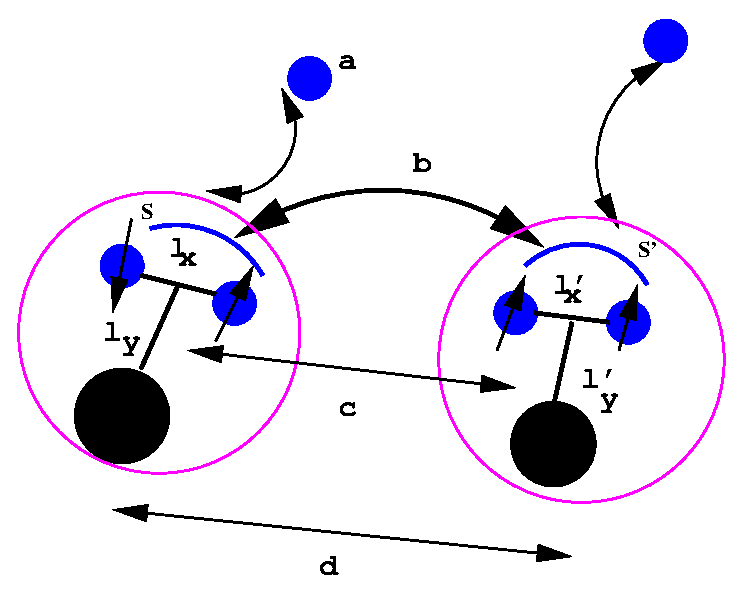
\includegraphics{spin_tensor.eps}} \par}
\caption{\label{Fig:spin_tensor}
Scattering quantum numbers }
\end{figure}
%%%%%%%%%%%%%%%%%%%%%%%%%%%%%%%%%%%%%%%%%%%%


For the particular case of a central interaction then
\be
\hat{t}_{[0 0 {\cal S}_p  {\cal S}'_p ]}(\omega_{01},\vec{\Delta}) =
 t^{(00)}_{00}(\omega_{01} \, , \vec{\Delta }) 
\ee
and the density formfactor for elastic scattering is
\be
\rho _{[0 0 ; {\cal S}_T {\cal S}'_T \hat{\epsilon}_0]}
\left( \frac{m_2}{M_{12}}  ,\frac{M_{3}}{M_{123}}\vec{\Delta }\right)
=   \hat{\rho }_{[000]}^{J_0J_0 \hat{\epsilon}_0}
\left( 0,\frac{m_{3}}{M_{123}}{\Delta }\right)
\ee


\subsubsection{ Scattering from the core:}

The scattering from the core can be written as:
\be
\label{eq:sscatv}
\langle \vec{k}'_{0} \chi_{s_0}^{{\sigma}'};\Psi_{\hat{\epsilon}_i}^{J M}
|\hat{t}_{13}|\vec{k}_{0}\chi_{s_0}^{\sigma} ;\Psi_{0}^{J_0 M_0}  \rangle
  = 
\hat{t}_{[0 0 {\cal S}_p  {\cal S}'_p ]} (\omega_{13},\vec{\Delta})
\times  \rho_{[0 0 ; {\cal S}_T {\cal S}'_T \kappa_i]}
\left(0,\frac{m_3}{m_{12}}\vec{\Delta }\right)
\nonumber \\
\ee
 The amplitude
$ \hat{t}_{[b \beta {\cal S}_p  {\cal S}'_p ]}$
is given in terms of the tensor components of the nucleon-nucleon
transition amplitude as
\be
\hat{t}_{[0 0 {\cal S}_p  {\cal S}'_p ]}(\omega_{03},\vec{\Delta})
  =  \sum _{ a\alpha }(-)^{\alpha} 
\langle s_0|| \tau _{a}(\frac{1}{2};0) || s_0\rangle 
  \times   t^{(a0)}_{a \alpha}(\omega_{03} \, , \vec{\Delta })
(s_0\sigma a\alpha |s_0\sigma ')
\ee
The density formfactor is
\be
\rho _{[0 0 ; {\cal S}_T {\cal S}'_T \hat{\epsilon}_i]}
\left(0,\frac{M_{12}}{M_{123}}\vec{\Delta }\right)
=  \sum \hat{\rho }_{[0cc]}^{JJ_0 \hat{\epsilon}_i}
\left( 0,\frac{M_{12}}{M_{123}}{\Delta }\right)
 \times  \hat{\varrho }_{[0 0 cc]}^{JM J_0M_0 }(\hat{\Delta }) \label{rho1}
\ee
For the particular case of a central interaction then
\be
\hat{t}_{[0 0 {\cal S}_p  {\cal S}'_p ]}(\omega_{03},\vec{\Delta}) =
 t^{(00)}_{00}(\omega_{03} \, , \vec{\Delta }) 
\ee
and the density formfactor for elastic scattering is
\be
\rho _{[0 0 ; {\cal S}_T {\cal S}'_T \hat{\epsilon}_0]}
\left(0,\frac{M_{12}}{M_{123}}\vec{\Delta }\right)
=  \hat{\rho }_{[000]}^{J_0J_0 \hat{\epsilon}_0}
\left( 0,\frac{M_{12}}{M_{123}}{\Delta }\right)
\ee


\subsection{Relativistic kinematics}
Within MST, the projectile-target scattering scattering amplitude
is constructed from the projectile-subsystem scattering amplitude
as described in the text. We shall discuss  the relativistic kinematics
for the scattering of both the  composite and each subsystem.

Let us  consider the elastic scattering of projectile 
labelled '0' with a target '$A$'.
In our case $A$ represents a composite  system.
We denote respectively $m_0$ and $m_A$ the rest mass of particles 0 and A,
and in here ${\cal K}_0$ and ${\cal K}_A$ ($\vec{\cal K}_0$, $\vec{\cal K}_A$)
their four-momenta (three-momenta)
\be
{\cal K}_i^2 = E_i^2 - \vec{\cal K}_i^2 = m_i^2 ~~~,~~ 0=1,A ~~.
\ee
In relativistic kinematics one introduces
the Lorentz invariant Mandelstam variable \cite{Joa87}
\be
s_{0A} &=&  \left( {\cal K}_0  + {\cal K}_A \right)^2 
= (E_0 + E_A)^2 - ( \vec{\cal K}_0 +  \vec{\cal K}_A )^2
\ee
In the laboratory frame, where $\vec{\cal K}^{\rm Lab}_A = 0$, 
the Mandelstam invariant is
\be
s_{0A} = m_{A}^2 + {m}_0^2 + 2 {m}_{A}  T^{\rm Lab} ~~,
\label{MandelstamLAB}
\ee
with $T^{\rm Lab} = \sqrt{m_0^2 + \left({\vec{\cal K}}^{\rm Lab}_0\right)^2}$. 
Alternatively,  in the projectile-target CM frame where
$ \vec{\cal K}^{\rm CM}_0 = \vec{k}_0, \vec{k}^{\rm CM}_A=-\vec{k}_0$ one has
\be
s_{0A} &=& \left( E_0 + E_A \right)^2  \nonumber \\     
&=& \left( \sqrt{m_0^2 + \vec{k}_0^2} +  \sqrt{m_A^2 + \vec{k}_0^2}
\right)^2 ~~.
\label{MandelstamCM}
\ee
It follows from Eq.~(\ref{MandelstamCM}) that in the CM frame, the energies
are related to the Mandelstam invariant as
\label{ffromT}
\be
E_0=\frac{1}{2\sqrt{s_{0A}}}(s_{0A}+{m}_0^2  - {m}_A^2 ) ~~, \\
E_A=\frac{1}{2\sqrt{s_{1A}}}(s_{0A}-{m}_0^2  + {m}_A^2 )~~.
\ee
The differential cross section for projectile-target with respect to 
the four momentum transfer $t_{0A}$ is related to 
the c.m. differential cross section according to 
\be
\frac{d \sigma}{d t_{0A}} = \frac{ \pi}{k_0^2} \frac{d \sigma}{d \Omega}
\ee
where $t_{0A}=-|\Delta|^2 = 2 k_0^2 (\cos \theta_{\rm c.m.} - 1) $  
and $k_1$ the projectile momentum in the CM frame, which can
be obtained from the Mandelstam variable Eq.~(\ref{MandelstamCM})
\be
k_0 = 
\frac{\left[s_{0A} - ({m}_{A} + {m}_0)^2 \right]
 \left[s_{0A} - ({m}_{A} - {m}_0)^2 \right] }
{4 s_{0A}} ~~.
\label{Crelativistic}
\ee
This expression reduces to 
\be
k_0 = \sqrt{\frac{2 \mu_{0,A} E_0}{\hbar^2} }
\label{Cnonrelativistic}
\ee
in the nonrelativistic case. The cross section is evaluated from
the scattering amplitude,  related to the matrix elements of
the total transition amplitude according to \cite{Joa87}
\be 
F &=& \frac{(2 \pi^2)^4}{\hbar v_0} k_0^2 
\frac{dk_0}{d E} \langle  \vec{k}\,'_0 | T(\omega) |  \vec{k}_{0}\rangle
\label{Frelativistic}
\ee
with 
\be
\omega=(E_0+E_A)=\sqrt{s_{0A}} - m_0 - m_A~~,
\ee

%=======================================================
Let us  consider now the projectile  scattering from subsystem ${\cal I}$.
As before, we introduce the Mandelstam variable for the interacting pair:
\be
s_{0{\cal I}} &=& (E_0 + E_{\cal I})^2 
- ( \vec{\cal K}_0 +  \vec{\cal K}_{\cal I} )^2
\ee
For simplification, we shall take the relative momentum of the interacting 
subsystems nonrelativistically and equal to zero.
Then  in the laboratory frame  
the Mandelstam variable $s_{1{\cal I}}$ can be readily evaluated 
\be
s_{0{\cal I}} = {m}_{0}^2  + {m}_{\cal I}^2 
+ 2 {m}_{\cal I} ({m}_0  + T^{\rm Lab}) ~~.
\ee
From the evaluated  Mandelstam invariant  $s_{0{\cal I}}$, the projectile $E_0$
and subsystem $E_{\cal I}$ energies are constructed according to
\be
E_0=\frac{1}{2\sqrt{s_{0{\cal I}}}}(s_{0{\cal I}}+{m}_0^2  - {m}_{\cal I}^2 )\\
E_{\cal I}=\frac{1}{2\sqrt{s_{0{\cal I}}}}
(s_{0{\cal I}}-{m}_0^2  + {m}_{\cal I}^2 )
\ee
and hence the two-body energy parameter
\be
\omega_{0{\cal I}}=(E_0+E_{\cal I})=\sqrt{s_{0{\cal I}}} - m_0 -m_{\cal I} ~~,
\ee
and the relative momenta between the interacting pair
\be
{\cal Q}_{0{\cal I}}^2 &=& (E_0^2 - m_0^2 )
\label{3momentum-2body}
\ee
In the non-relativistic case  
${\cal Q}_{1{\cal I}}^2 = \frac{2 \mu_{0{\cal I}} E_0}{\hbar^2}$.
The differential cross section for the scattering from subsystem
${\cal I}$ with respect to the four momentum transfer
$t_{0{\cal I}}$,  is related to the c.m. differential cross section as:
\be
\frac{d \sigma}{d t_{0{\cal I}}} = \frac{\pi}{{\cal Q}_{0{\cal I}}^2} 
\frac{d \sigma}{d \Omega}_{0{\cal I}}
\ee
where $t_{0{\cal I}} = 2 {\cal Q}_{0{\cal I}}^2(\cos \theta_{0,{\cal I}} - 1)$.
The elastic scattering amplitude is related to the T-matrix elements through:
\be 
f_{\cal I} = \frac{(2 \pi^2)^4}{\hbar v_0} k_0^2
\frac{dk_0}{d \omega_{0{\cal I}} } 
\langle {\cal \vec{Q}'}_{0{\cal I}} | \hat{t}_{\cal I} 
(\omega_{0 {\cal I}})| 
{\cal \vec{Q}}_{0 {\cal I}}\rangle
\label{f2relativistic}
\ee

\section{Running SAM}


\subsection{Source files}

The \textbf{SAM} source files are organized into three directories,
\emph{nnrc, msosrc} and \emph{mstrc}. The former contains the NNamp
source files, while msorc and mstrc contain those files specific of
the MSOamp and MSTamp formalisms respectively. 


\paragraph*{\emph{NNamp sources}}

%%%%%%%%%%%%%%%%%%%%%%%%%%%%%%%%%%%%%%%%%%%%%%%%%%%%%%%%%%%%%%%%%%%%%%%%%%%%%%%
\begin{figure}
{\centering \includegraphics{nn_plan.eps} \par}
\caption{\label{Fig:mat_plan }NN main subroutines general chronogram}
\end{figure}
%%%%%%%%%%%%%%%%%%%%%%%%%%%%%%%%%%%%%%%%%%%%%%%%%%%%%%%%%%%%%%%%%%%%%%%%%%%%%



\begin{itemize}
\item \textbf{main.f90}: main program, reads the input file and calls to
the different subroutines.
\item \textbf{klsp.f90}: program to build the R-matrix for uncoupled states. 
\item \textbf{ktall.f90}: program to build the T-matrix, by solving the
Heitler equation.
\item \textbf{ampon.f90}: program to evaluate \emph{on-shell} amplitudes
in the Wolfenstein representation.
\item \textbf{ampall.f90}: program to evaluate \emph{off-shell} amplitudes
in the Wolfenstein representation.
\item \textbf{mon.f90}: program to evaluate \emph{on-shell} amplitudes in
the tensor representation.
\item \textbf{moff.f90}: program to evaluate \emph{off-shell} amplitudes
in the tensor representation.
\item \textbf{utils.f90}: subroutines of general use, shared by several
source files.
\begin{itemize}
\item \textbf{   sim(fa,res,m,n,h)}: 
 subroutine that evaluates the integral of {\em fa} stored
 in the arrays of the same name using Simpson rule. The step lenght
 is {\em h} and the integral is between the elements {\em m} and {\em n} of the array
 only. The resulting integral is placed in {\em res}.
 \item \textbf{gauss2(npts, kode, a, b, xs, wts)}:
subroutine that calculates quadrature 
points {\em xs} and weights {\em wts}. 
The number of points is {\em npts} (must be 8, 16, 24, 32, 40, 48).
The {\em kode} (standard=022) is a 3-digit decimal number written as 
{\bf htu} with the digits having the following functions: 
{\bf h}=0(no special action), =1(a square root singularity is removed 
from the choice of the points at the lower limit of the integral);
{\bf t} =1 (the interval is {\em a} to {\em b} where {\em b} 
may be less than {\em a}) 
=2 (the interval is 0 to $\infty$ with 50 $\%$ of the points on 
(0,{\em a}) and 50 $\%$ of the points on [{\em a},$\infty$], {\em b} 
is not used);
=3 (the interval is from  $- \infty$ to  $+ \infty$ with 50 $\%$ 
of the points on [-{\em a},{\em a}], {\em b} is not used);
=4 (the interval is {\em b} to $\infty$ with 50 $\%$ of 
the points on [{\em b}, {\em a} + 2{\em b})]);
=5 (the interval is 0 to {\em b} with 50 $\%$ of the points on 
[0,{\em a}{\em b}/({\em a}+{\em b})]). 
{\bf u} are the type type of Gauss-Legendre points
 =0 (requires 8, 16, 24, 32, 40, 48);
 =2 (changes npts to the next larger value);
 =5 returns equal -spaced points according to the Simpson's 
rule if {\em npts} is odd.
\item \textbf{gauss3(rmaxr,quin,mquadi,mquado,xri,wri)}: 
subroutine that calculates quadrature 
points {\em xri}, and weights {\em wri}  in {\em mquadi}  steps of equal size 
from 0 to {\em quin}, and quadrature points in {\em mquado}  steps 
of linerly size from {\em quin} to {\em rmaxr}.
%%%%%%%%%%%%%%%%%% Interpolation
\item  \textbf{ fival(r,xv,fdis,ndm,alpha)}: 
real 4-point lagrange interpolation 
of the function value {\em fival} at point {\em r} from an
array of points stored in {\em fdis(ndm)}. This array is assumed
to be defined such that the first element {\em fdis(1)} contains
the function value at {\em r=xv(1)} and {\em xv(2 .. ndm)} are monotonically
increasing.
\item  \textbf{  lagrng(x,arg,y,val,ndim,nfs,nptx,maxarg,maxfs)}:
lagrange interpolation,unequally spaced points
npts=2,3,4,5,6, nfs functions (y*s) simultaneously interpolated.
x= value of argument, arg is the tabulated x*s;
y= a vector of interpolated functions, from tabulted val;
ndim= dimension of table;
nfs =  of functions simult interpolated;
maxarg and maxfs are maximum values of subscripts,ie dimensions.
\item \textbf{ cint2d(xtab,ytab,fxytab,xbar,ybar,nnx,nny,nord,mmx)}: 
two dimensional complex  interpolation routine. It is assumed that the 
 mesh points are given in increasing order. 
The complex matrix {\em fxytab(xbar,ybar)} is interpolated at the
 point {\em (xtab,ytab)}. 
The vectors {\em xbar,ybar} have  {\em nnx,nny} points
respectively; {\em mmx} is the maximum value of  {\em nnx,nny}; {\em nord = 5}.
%%%%%%%%%
\item \textbf{ cmatin(a, b, n)}: 
subroutine that  finds the inverse of complex matrix 
h=(real,imag)=({\em a},{\em b}) of dimension {\em n}.
%%%%%%%%% Legendre polynomials
\item \textbf{legpol(x, plofx, n)} 
subroutine that calculates legendre polynomial using recurrence formula
\item \textbf {plprme (x, plp, n)}: 
subroutine that calculates the derivative of the legendre polynomials
\item \textbf{pldblp(xx,y,n)}: 
calculates the second derivative of the legendre polynomial.
%%%%%%%%% Bessel
\item \textbf{bessj(n,x)}: calculates bessel function 
\item \textbf{bessjy(x,xnu,rj,ry,rjp,ryp) }:
calculates bessel function {\em rj}, {\em ry} 
and their derivatives {\em rjp}, {\em ryp}.
%%%%%%%% Coulomb
\item \textbf{sigcl(som,sc,lmax); sigcl3(eta,scou,lmax);  coul(eta,cph,lmax)}: 
subroutines that calculate the coulomb phase shift  up tp {\em lmax}.
\end{itemize}
\item \textbf{modules.f90}: common modules.
\item \textbf{modbonn.f90}: modules associated to the construction of the
Bonn potential.
\end{itemize}

\paragraph*{\emph{MSOamp sources}}

%%%%%%%%%%%%%%%%%%%%%%%%%%%%%%%%%%%%%%%%%%%%%%%%%%%%%%%%%%%%%%%%%%%%%%%%%%%%%%%
\begin{figure}
{\centering \includegraphics{mso_plan.eps} \par}
\caption{\label{Fig:mat_plan }MSO general main subroutines chronogram}
\end{figure}
%%%%%%%%%%%%%%%%%%%%%%%%%%%%%%%%%%%%%%%%%%%%%%%%%%%%%%%%%%%%%%%%%%%%%%%%%%%%%


\begin{itemize}
\item \textbf{msomain.f90}: main program
\item \textbf{rc1.f90}: program that 
 reads the input file and calls to the different subroutines
\item \textbf{rc2.f90}: 
program that calculates scattering amplitudes for nucleon-proton and 
nucleon-neutron scattering and the formfactor for full folding calculations 
from a double closed shell nucleus.
\item \textbf{rc3.f90}: 
program that calculates second order optical potential for $^{16}$O
\item \textbf{rc4.f90}: 
program that calculates the partial wave expansion of 
elastic scattering wavefunction 
\item \textbf{optpot.f90}:
 program that solves the Lippmann-Schwinger equation from the
optical potential
\item \textbf{formf.f90}: 
program to calculate the  analytical density form factor: HO, 
Three-parameter free, G3 density distribution and the optical potential
\item \textbf{ffact.f90}: 
program to calculate the numerical density form factor for
a single particle in a  potential of type:  Woods-Saxon, Gauss, Yukawa,
Hulthen and Cosh
\item \textbf{xsec.f90}: 
program that calculates the elastic scattering observables
\item \textbf{modules.f90}: common modules
\end{itemize}

\paragraph*{\emph{MSTamp sources}}

\begin{itemize}
\item \textbf{mstmain.f90}: main program that
reads the input file and calls to the different subroutines
\item \textbf{read3bwf.f90}: program that reads target wave function
\item \textbf{readsmat.f90}: program that reads external s-matrix for the scattering from 
the core
\item \textbf{modmst.f90} common modules
\item \textbf{mstutils.f90} subroutines of general use, shared by several
source files.
\end{itemize}

%%%%%%%%%%%%%%%%%%%%%%%%%%%%%%%%%%%%%%%%%%%%%%%%%%%%%%%%%%%%%%%%%%%%%%%%%%%%%%%%%%%%%%%%
\begin{figure}
{\centering 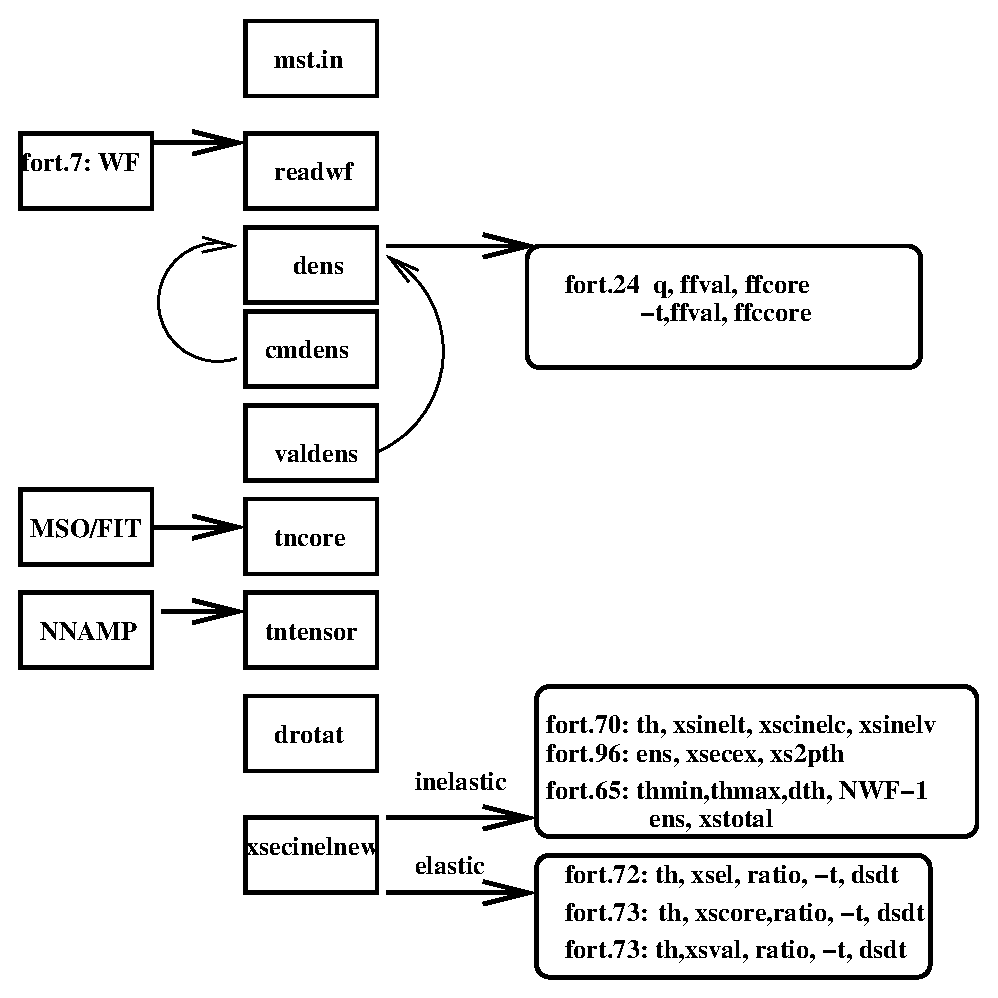
\includegraphics{mst_plan.eps} \par}
\caption{\label{Fig:mat_plan }MST main subroutines general chronogram}
\end{figure}
%%%%%%%%%%%%%%%%%%%%%%%%%%%%%%%%%%%%%%%%%%%%%%%%%%%%%%%%%%%%%%%%%%%%%%%%%%%%%%%%%%%%%%%%%



\paragraph{\emph{Utilities sources}}

\begin{itemize}
\item \textbf{Dfold.f90}: program that calculates a double folding potential from
realistic NN transition amplitudes and external densities for projectile and
target.
\item \textbf{Espectrum.f90} program that calculates the energy spectrum from the 
double differential cross section.
\item \textbf{Fit.f90}
\end{itemize}

\subsection{Source files and compilation}

Each of the three \textbf{SAM} main directories, \emph{nnrc} and \emph{msosrc}
and \emph{mstrc} directories contains a Makefile. There exits also
a Makefile in the top directory of the distribution. If needed, this
can be edited and customized before compilation. Notice that the compiler
name and options are included by means of {*}.def files. Presently,
two of these files are included: \emph{fujitsu.def} and \emph{pgf90.def}.
They contain the compilation specifications for the Fujitsu and PGF90
compilers, respectively. If one has a different f90 compiler, it is
necessary to create a {*}.def file, with the appropriate options. 

Once the top Makefile have been customized, the NNamp program can
be compiled with:

\begin{verbatim}prompt> cd nnsrc ; make\end{verbatim}

Similarly, to compile the MSOamp program:

\begin{verbatim}prompt> cd msosrc; make\end{verbatim}

Alternatively, from the top directory to can compile the NNamp program
typing:

\begin{verbatim}prompt> make nnamp \end{verbatim} 

\noindent and the MSOamp program with:

\begin{verbatim}prompt> make msoamp \end{verbatim} 

Notice that, whenever the MSO program is compiled, the NNamp program
will also be compiled. 

After compilation, you can delete the {*}.o files by typing: 

\begin{verbatim}prompt> make clean \end{verbatim}

To delete {*}.o as well as MSOamp / NNamp output files: 

\begin{verbatim}prompt> make superclean \end{verbatim}

To install the executables in the compilation (mso and nnamp) into
the destination specified at the top Makefile, type:

\begin{verbatim}prompt> make install \end{verbatim}


\section{Description of namelists input variables}


\subsection{NNamp.in}


\subsubsection*{SYSTEM namelist: }

The energy and NN realistic potential

\begin{itemize}
\item \textbf{tcm} (real): c.m. scattering energy.
\item \textbf{nnpot} (string): type of NN interaction. Currently 'Paris'
or 'Bonn'.
\item \textbf{jmax} (integer): if specified the set of partial waves \( L,S,J \)
will be built automatically. Otherwise, a set of \&pw/ namelists are
required to explicitly input the desired partial waves. 
\end{itemize}

\subsubsection*{KMAT namelist:}

Variables necessary to evaluate the integral over the transferred
momentum, \( q \), for constructing the R-matrix. The integration
is done by dividing the integration interval into four pieces, with
(see Fig.\ \ref{Fig:redish})

\begin{itemize}
\item \textbf{hw}: half-width of (symmetric) interval around the on-shell
value (default 0.5).
\item \textbf{b01,} \textbf{b34}: lower and upper limits.
\item \textbf{n1,n2},\textbf{n3, n4}: number of quadrature points in each
one of the regions.
\item \textbf{s}: scale factor for Gauss-Laguerre quadrature (default 1).
\item \textbf{qlo}: lowest momentum (default 0).
\item \textbf{qhi}: highest momentum (default 1000).
\begin{figure}
{\centering \includegraphics{redish.eps} \par}


\caption{\label{Fig:redish}Integration intervals for the evaluation of the
R-matrix}
\end{figure}

\end{itemize}

\subsubsection*{OUT namelist:}

Magnitudes to be printed out.

\begin{itemize}
\item \textbf{dels}: phase shifts.
\item \textbf{aeoff}: off-shell amplitudes in the Wolfestein parametrization.
\item \textbf{aeon}: on-shell amplitudes in the Wolfestein parametrization.
\\
\\
\begin{tabular}{|c|c|c|}
\hline 
\multicolumn{3}{|c|}{aeoff}\\
\hline
Value&
Written amplitudes&
Unit\\
\hline
\hline 
0&
-&
-\\
\hline 
1&
Isoscalar&
22\\
&
Isovector&
23\\
\hline 
2&
T=0&
34\\
&
T=1&
33\\
\hline 
3&
pn&
32\\
\hline
\end{tabular}~~~~\begin{tabular}{|c|c|c|}
\hline 
\multicolumn{3}{|c|}{aeon}\\
\hline 
Value&
Writen amplitudes&
Unit\\
\hline
\hline 
0&
-&
-\\
\hline 
1&
Isoscalar&
220\\
&
Isovector&
230\\
\hline 
2&
T=0&
340\\
&
T=1&
330\\
\hline 
3&
pp&
320\\
\hline
\end{tabular} \\
\\
Al these files have the format: \\
\\
\begin{tabular}{cccccccc}
$\theta$ &
Re(\( \cal {A} \))&
Img(\( \cal {A} \))&
Re(\( \cal {B} \))&
Img(\( \cal {B} \))&
\ldots{}&
Re(\( \cal {F} \))&
Img(\( \cal {F} \))\\
\end{tabular} \textbf{}
\item \textbf{moff}: off-shell amplitudes in tensor representation. Using
the notation of \cite{Cres01}, the following six independent amplitudes
are written: \( M_{00}^{(00)} \), \( M_{11}^{(01)} \), \( M_{00}^{(11)} \)
\( M_{20}^{(11)} \), \( M_{21}^{(11)} \) and \( M_{22}^{(11)} \)
. The names of the output files are built as:\[
M^{ab}_{kq}\, \rightarrow \, \mathrm{mabkq}.\mathrm{off}\]
The possible values of the variable \emph{moff} are: \\
\\
\begin{tabular}{|c|cc|}
\hline 
\multicolumn{3}{|c|}{moff}\\
\hline
\hline 
Value&
\multicolumn{2}{c|}{Written amplitude}\\
\hline 
0&
\multicolumn{2}{c|}{No output}\\
\hline 
1&
Isoscalar &
Isovector\\
\hline 
2&
T=0 &
T=1\\
\hline 
3&
pn  &
pp\\
\hline
\end{tabular}\\
\\
For each of the components, real and imaginary parts are written in
consecutive columns.
\item \textbf{mon}: on-shell amplitudes in tensor representation. The filenames
are the same, but using the extension \emph{.on}
\end{itemize}

\subsubsection*{PW namelist:}

Partial waves. 

\begin{itemize}
\item \textbf{is}: total spin of the NN system (0,1), S. 
\item \textbf{ll}: total orbital angular momentum, L.
\item \textbf{jj}: total angular momentum, J.
\end{itemize}

\subsubsection*{AMP namelist: }

Extra variables necessary to build the momentum space grid.

\begin{itemize}
\item \textbf{ifkq}: definition of the momentum transfered \( q \) and
total momentum \( Q \).
\end{itemize}
{\centering \begin{tabular}{|c|cc|}
\hline 
ifkq=0&
\( \vec{q}=\frac{\mathcal{K}'-\mathcal{K}}{\sqrt{2}} \) &
\( \vec{Q}=\frac{\mathcal{K}'+\mathcal{K}}{\sqrt{2}} \)\\
\hline
ifkq=1&
\( \vec{q}=\mathcal{K}'-\mathcal{K} \)&
\( \vec{Q}=\frac{\mathcal{K}'+\mathcal{K}}{2} \)\\
\hline
\end{tabular}\par}

\begin{itemize}
\item \textbf{xkmax}=step in \( Q \).
\item \textbf{xqmax}=step in \( q \).
\item \textbf{dk}: step in \( Q \) (default 0.1). 
\item \textbf{dq}: step in \( q \) (default 0.1) .
\item \textbf{theta}: angle between \( \vec{q} \) and \( \vec{Q} \), in
degrees (default 90).
\item \textbf{nth}: number of angles to calculate on-shell values (default
46). 
\end{itemize}

\subsection{MSO.in}


\subsubsection*{MSO namelist: }

\begin{itemize}
\item \textbf{tlab}: relative kinetic energy projectile-target in laboratory
system.
\item \textbf{offshell}: T/F
\item \textbf{kmt}: KMT (kmt=T) or Watson (kmt=F) potential. The former
contains the multiplying factor at/(at-1), with at the target atomic
number.
\item \textbf{lxmax}: maximum number of projectile-nucleus orbital angular momentum
\item \textbf{ngp}: number of grid points used in discretizing the Lipppmann-Schwinger integral
       equation (must be 8, 16, 24, 32, 40 or 48)
\item \textbf{kode}: (standard=022) is a 3-digit decimal number written as {\bf htu} with the
digits having the following functions: {\bf h}=0(no special action), =1(a square
root singularity is removed from the choice of the points at the lower limit of the integral);
{\bf t} =1 (the interval is {\em a} to {\em b} where {\em b} may be less than {\em a}) 
=2 (the interval is 0 to $\infty$ with 50 $\%$ of the points on (0,{\em a}) and  
 50 $\%$ of the points on ({\em a},$\infty$). {\em b} is not used.)
=3 (the interval is from  $- \infty$ to  $+ \infty$ with 50 $\%$ of the points on (-{\em a},{\em a}.
{\em b} is not used.)
=4 (the interval is {\em b} to $\infty$ with 50 $\%$ of the points on [{\em b}, {\em a} + 2{\em b})]. )
=5 (the interval is 0 to {\em b} with 50 $\%$ of the points on[0,{\em a}{\em b}/({\em a}+{\em b})].) 
{\bf u} are the type type of Gauss-Legendre points. = 0 (requires 8,16,24,32,40,48)
=2 (changes npts to the next larger value)
=5 returns equal -spaced points according to the Simpson's rule if {\em ngp} is odd.
\item \textbf{b}: mid point value of the grid
\item \textbf{nang}: angular stepsize in degrees for which the differential equation over the 
interval (0,180) are to be computed
\item \textbf{ymin1}: not used
\item \textbf{ymin2}: not used
\item \textbf{nr}: if nr is not 0, relativistic kinematics is used. 

\end{itemize}

\subsubsection*{COUL namelist:}

\begin{itemize}
\item \textbf{coulomb}: Coulomb correction\\
=0: no coulomb\\
=1: coulomb amplitude and phase change included~\\
=2: coulomb amplitude, but not phase change\\
=3: subtracted method with realistic (HO shape) charge distribuion\\
=4: subtracted method with realistic (uniform charged sphere) charge 
     distribution
\item \textbf{rcut}: cut-off radius for subtracted momentum space method
\cite{Crespo90}.
\item \textbf{alfa, beta, gama}: parameters for the realistic 
charge distribution of  Harmonic Oscilator  form:
\begin{equation}
\rho (q)=\left\{ 1-\gamma ^{2}q^{2}+\alpha q^{4}\right\} e^{-\beta q^{2}}
\end{equation}

\end{itemize}

\subsubsection*{HIGHORDER namelist:}

Specifications for high order calculations (second order onward)

\begin{itemize}
\item \textbf{second}:\\
= 1 SSA\\
= 2 DSA(local)\\
= 3 DSA (non local) \\
= 4 DSA (full nonlocal)
\item \textbf{isflip}:= 0 only isoscalar central, 
      = 1 all 10 isoscalar and isovector on-shell scattering amplitudes
\item \textbf{ich}: = 0
\item \textbf{ion2}:Not used 
\item \textbf{lamx}: maximum value of the radial angular momentum of the single
              particle states 
\item \textbf{lbmx}:  maximum value of the radial angular momentum of the 
                single particle states 
\item \textbf{l1mx}: number of partial waves to be calculated in the 
      nonlocal and full nonlocal second order potential
\item \textbf{lfmx}: maximum number of multipoles of the NN 
     scattering  matrix elements to be calculated in the full nonlocal 
     second order potential
\item \textbf{rmaxr}: maximum radius
\item \textbf{quin}: maximum radius for inner region
\item \textbf{mquadi}: number of inner quad points (multiple of 6)
\item \textbf{mquado}: number of outer quad points (multiple of 6)
\end{itemize}

\subsubsection*{PROJ namelist:}

Projectile properties. Presently, the program only supports structureless
projectiles. Thus, unlike the target, no clusters can be defined.

\begin{itemize}
\item \textbf{massp}: mass number (in a.m.u.)
\item \textbf{zp}: charge
\end{itemize}

\subsubsection*{TARG namelist:}

Target properties

\begin{itemize}
\item \textbf{masst}: mass number (in a.m.u.)
\item \textbf{zt}: charge
\item \textbf{at}: number of nucleons
\item \textbf{ncluster}: number of clusters
\end{itemize}

\subsubsection*{CLUSTER namelist:}

After the \textbf{targ} namelist, \emph{ncluster} namelists will be
read. Each one contains the information required to construct the
density for one the clusters. Notice that the different cluster do
not necessary have to use the same model density.

\begin{itemize}
\item \textbf{type}, \textbf{shape}: specify the kind of density. External
densities (type=1, shape=5) are read from fortran unit 4. The first
line contains the number of points (\emph{nramax}) and the step (\emph{drx}),
in free format. Then, nramax density points will be read, assuming
that the first one corresponds to the origin. \\
\begin{tabular}{|cc|cl|}
\hline 
\multicolumn{2}{|c|}{type}&
\multicolumn{2}{c|}{shape}\\
\hline
\hline 
0&
Numerical potential&
0&
Woods-Saxon\\
&
&
1&
Gauss\\
&
&
2&
Yukawa\\
&
&
3&
Hulthen\\
&
&
4&
cosh\\
&
&
5&
External\\
\hline 
1&
Analytical potential&
0&
Harmonic-oscillator s.p.\\
&
&
1&
Three-parameter Fermi\\
&
&
2&
G3 distribution\\
\hline
\end{tabular}
\item \textbf{nzclus}: number of protons within this cluster.
\item \textbf{nnclus}: number of neutrons within this cluster.
\end{itemize}

\subsubsection*{BSPARM namelist:}

For type=0, shape=0-4 the bsparm namelist is then read.

\begin{itemize}
\item \textbf{cmass, vmass}: core and bound particle masses.
\item \textbf{zc, zv}: core and bound particle charges.
\item \textbf{nramax}: number of integration steps.
\item \textbf{drx}: radial step for numerical integration.
\item \textbf{dmat}:fine tuning of interior-exterior matching. Usually input
0. {*} If no state found try increase of dmat to of order 10.
\item \textbf{nshell}: number of shells.
\end{itemize}

\subsubsection*{BSHELL namelist:}

Parameters for this specific shell.

\begin{itemize}
\item \textbf{bengy}: binding energy.
\item \textbf{vdepth}, \textbf{wr0, wal}: potential depth, radius and diffuseness.
\item \textbf{wls}: spin-orbit strength.
\item \textbf{is2}=2{*}valence particle spin \( s \).
\item \textbf{lmoma}= orbital angular momentum \( \ell  \).
\item \textbf{j2a} : 2{*}j, where \( j=\ell +s \).
\item \textbf{nodd}=number of nodes.
\item \textbf{norba}=occupation number of this shell.
\end{itemize}

\subsubsection*{BS3PF namelist:}

If type=1, shape=5 density is defined, a \textbf{\&bs3pf/} namelist
is then read. In configuration space, it obeys to the form:\begin{equation}
\label{Eq:rho-fermi}
\rho (r)=\rho _{0}\frac{1+w(r/c)^{2}}{\exp [(r-c)/z]}
\end{equation}
where \( \rho _{0} \) is a normalization constant and \( w,\, c,\, z \)
are free parameters. 

\begin{itemize}
\item \textbf{w3p, z3p}, \textbf{c3p}: Fermi parameters for protons.
\item \textbf{w3n, z3n, c3n}: Fermi parameters for neutrons.
\item \textbf{nramax}: number of radial points to calculate the density.
\item \textbf{drx}: step size (fm).
\end{itemize}

\subsubsection*{HOPARM namelist:}

For type=1, shape=0 densities, harmonic oscillator parameters are
read. First, a \textbf{hoparm} namelist is introduced, which currently
only contains the number of shells that will be next read by means
of \textbf{hoshell} namelists.

\begin{itemize}
\item \textbf{hoparm}: number of harmonic-oscillator shells to be read.
\end{itemize}

\subsubsection*{HOSHELL namelist: }

Provides the HO parameters and occupations numbers for each shell.

\begin{itemize}
\item \textbf{aap, aan}: HO parameters for protons and neutrons, respectively.
\item \textbf{zorba, norba}: occupation number (protons and neutrons) for
this shell.
\end{itemize}

\subsection{MST.in}


\subsubsection*{MST namelist:}

\begin{itemize}
\item \textbf{qmax: } Maximum value of momentum transfered $\Delta_max$ to evaluate the density
form factors. The number of points is qmax/ndel with ndel=25.
\item \textbf{tlab}: projectile energy in laboratory frame.
\item \textbf{thmin, thmax, dth}: angular range and step for calculated
cross sections.
\end{itemize}

\subsubsection*{QUAD1 namelist:}
\textbf{qmaxr}, 
\textbf{quin}, 
\textbf{mquadi}, 
\textbf{mquado}: Not used


\subsubsection*{QUAD2 namelist:} Gauss2 quadrature data for setting momentum transfer points and weights 
\begin{itemize}
\item \textbf{qmaxrd}: outer transfered momentum  point
\item \textbf{quind}: inner transfered momentum  point
\item \textbf{mquadid:}  Number of quadrature points from 0 to {\em quind}
\item \textbf{mquadod}:  Number of quadrature points from {\em quind}  to {\em quind}
\end{itemize}

\subsubsection*{QUAD3 namelist:}
\textbf{rmaxr}, 
 \textbf{rin},
 \textbf{mrquadi}, 
\textbf{mrquado}:  Not used

\subsubsection*{PROJ namelist:}

\begin{itemize}
\item \textbf{massp}: projectile mass
\item \textbf{zp}: projectile charge
\end{itemize}

\subsubsection*{TARG namelist:}

\begin{itemize}
\item \textbf{masst}: target mass
\item \textbf{zt}: target charge 
\item \textbf{ncl}: number of clusters.
\item \textbf{inelcb}: Not used
\item \textbf{nustates}: total number of states.
\item \textbf{quais(1:nustates-1)}: vector array to select those \( J^{\pi } \)
(inelastic) components of the wavefunction that will be taken into
account in the calculations. \( quais(i)\neq 0 \) means that component
\( i \) will be included.
\item \textbf{irho}: Not used
\end{itemize}

\subsubsection*{KAPAS namelist:}

\begin{itemize}
\item \textbf{k0000, k1100, k0111, k1120, k1121, k1122}: If \emph{kabkq}=1
the tensor component \( t^{(ab)}_{\kappa q}(\omega \, \vec{\Delta }) \)
of the NN amplitude will be taken into account.
\end{itemize}

\subsubsection*{TCLUS namelist: }

\begin{itemize}
\item \textbf{mtclus}: mass of this cluster (u.m.a.)
\item \textbf{spin}: cluster intrinsic spin
\item \textbf{ztclus}: cluster charge
\end{itemize}


\newpage
\section{Test case and set up}

The namelist input style provides a very intuitive description of
the input file by itself. 


\subsection*{Example of NN input file}

\noindent
$\diamond$  nnamp.in:

\verbatiminput{examples/nnamp_example.in}


\noindent
$\diamond$  Detailed description:

\&system tcm=32.5 nnpot='paris' /

The first namelist (\textbf{\&system/}) sets the center of mass energy
of the colliding nucleons and the kind of NN potential. In this example
the variable \textbf{jmax} is not specified and so it is understood
that partial waves are to be given explicitly in this input file.
\\

\&out dels=1 aeon=0 aeoff=0 mon=1 moff=1 /

The namelist \textbf{out} specifies the information that is going
to be calculated and printed out by the program. In this example the
phase shifts (\textbf{dels=1}) and the isoscalar and isovector
components of the on- and off-shell NN amplitude in tensor representation.\\

\&kmat hw=0.5 b01=0. b34=30. ,n1=5 n2=6 n3=15 n4=6, s=1.0, qlo=0.,
qhi=1000. /

Then, namelist \textbf{\&kmat/} it is provided the parameters required
to calculate the R-matrix. In particular, the boundaries of the regions
defined in the integration (\textbf{b01}, \textbf{b34} and \textbf{hw})
as shown in Fig.\ \ref{Fig:redish}. Also the number of quadrature
points is given (n1,n2,n3,n4). \\


\&pw is=0 ll=0 jj=0 /

\&pw is=1 ll=1 jj=0 /

\&pw is=0 ll=1 jj=1 /

\&pw is=1 ll=1 jj=1 /

\&pw is=1 ll=0 jj=1 /

\&pw is=0 ll=2 jj=2 /

\&pw is=1 ll=2 jj=2 /

\&pw is=1 ll=1 jj=2 /

\&pw is=0 ll=3 jj=3 /

\&pw is=1 ll=3 jj=3 /

\&pw is=1 ll=2 jj=3 /

\&pw is=0 ll=4 jj=4 /

\&pw is=1 ll=4 jj=4 /

\&pw is=1 ll=3 jj=4 /

\&pw is=0 ll=5 jj=5 /

\&pw is=1 ll=5 jj=5 /

\&pw is=1 ll=4 jj=5 /

\&pw is=0 ll=6 jj=6 /

\&pw is=1 ll=6 jj=6 /

\&pw is=-1 ll=0 jj=0 / 

Then a set of namelist \&pw/ are read in order to provide the partial
waves considered.

~

\&amp ifkq=1 xkmax=2.0 xqmax=3.5 dk=0.2 dq=0.2 theta=45. nth=90, 

itype=2 icase=2 /

Finally, the \textbf{\&amp/} namelist gives the required parameters
for the evaluation of the T-matrix starting from the R-matrix.


%%%%%%%%%%%%%%%%%%%%%%%%%%%%%%%%%%%%%%%%%%%%%%%%%%%%%%%%%%%%%%%%%%%%%%%%%
\begin{figure}
{\par\centering \resizebox*{0.55\textwidth}{!}
{\includegraphics{nnrealA-elab65.eps}} \par}
\caption{\label{Fig:nnrealA-elab65}
 Real Isoscalar and isovector central Wolfenstein amplitude for 
E$_{\rm LAB}$=65 MeV      }
\end{figure}
%%%%%%%%%%%%%%%%%%%%%%%%%%%%%%%%%%%%%%%%%%%%%%%%%%%%%%%%%%%%%%%%%%%%%%%%%



\newpage

\subsection*{Example of MSO input files}

\subsubsection*{p+$^{40}$Ca @ 65 MeV}

\noindent
$\diamond$  mso.in 


\verbatiminput{examples/mso-pca40HO-e65.in}

\noindent
$\diamond$  Detailed description:\\

\&mso tlab=65 offshell=T kmt=T  lxmax=40 
       ngp=40, kode=022 b=21000. nang=-1 ymin1=-7. ymin2=-2. nr=0 /

The first namelist (\textbf{\&mso/}) sets the laboratory energy
\textbf{tlab}=65 of the colliding nucleon. 
It takes offshell NN transition amplitudes, \textbf{offshell}= T,
for the KMT optical potential, \textbf{kmt}=T.
The maximum number of projectile-nucleus orbital angular momentum is
\textbf{lxmax}=40.
The number of grid points used in discretizing the Lipppmann-Schwinger integral
equation is \textbf{ngp}=40.
Sets standard \textbf{kode}=022,with middle grid point \textbf{b}=21000.
Assumes nonrelativistic kinematics, \textbf{nr}=0.\\

\&coul coulomb=3 rcut=10.  alfa=0.18 beta=0.95 gama=0.95 /

The  namelist (\textbf{\&coul/}) includes Coulomb using the 
subtracted method with realistic 
Harmonic Oscillator charge distribuion,\textbf{coulomb}=3, 
with a cutoff radius,\textbf{rcut}=10, and parameters  
\textbf{alfa, beta, gama} for the HO charge distribution.\\


\&highorder second=1 closure=F rmaxr=10. quin=6. mquadi=120 mquado=48 /

The  namelist (\textbf{\& highorder/}) sets the single scattering approximation
to the optical potential \textbf{second}=1. The other parameters of the
namelist are not used.\\

\&proj massp=1.0072 zp=1 /

The  namelist (\textbf{\& proj/}) sets the mass of the proton projectile
\textbf{massp}=1.0072, and its charge  \textbf{zp}=1\\

\&targ ncluster=1 masst=40. at=40 zt=20 /

The  namelist (\textbf{\& targ/}) sets the properties of the target,
the number of clusters of nucleons, \textbf{ncluster}=1,
the mass of the target  \textbf{massp}=1.0072, and its charge  \textbf{zp}=1\\

\&cluster type=1 shape=0 nzclus=20 nnclus=20 /

The  namelist (\textbf{\& cluster/}) sets for each cluster the 
density formfactor. The type is analytical \textbf{type}=1, and
derived from an Harmonic oscillator wave function  \textbf{shape}=0.
For this cluster the naumber of protons is \textbf{nzclus}=20 and
the number of nucleons \textbf{nnclus}=20.\\

 \&hoparm   nshell=4  /

 \&hoshell  aap=1.95  aan=1.95 zorba=2 norba=2 /

 \&hoshell  aap=1.95  aan=1.95 zorba=6 norba=6 /

 \&hoshell  aap=1.95  aan=1.95 zorba=10 norba=10 /

 \&hoshell  aap=1.95  aan=1.95 zorba=2 norba=2 /

For the HO cluster the number of shells is specified in the
namelist (\textbf{\& hoparm/}) as \textbf{nshell}=4. The HO parameters
for each shell are specified in the namelist (\textbf{\& hoshell/}).


\subsubsection*{n+$^{40}$Ca @ 65 MeV}

\noindent
$\diamond$  mso.in 


\verbatiminput{examples/mso-nca40HO-e65.in}

\noindent
$\diamond$  Detailed description:\\

\noindent
$\diamond$  Results:\\

In Fig~(\ref{Fig:mso-n+40Ca-e65}) we show the calculated elastic scattering
diferential cross section for n+$^{40}$Ca at 65 Mev.

%%%%%%%%%%%%%%%%%%%%%%%%%%%%%%%%%%%%%%%%%%%%%%%%%%%%%%%%%%%%%%%%%%%%%%%%%
\begin{figure}
{\par\centering \resizebox*{0.55\textwidth}{!}
{\includegraphics{mso-n+40Ca-e65.eps}} \par}
\caption{\label{Fig:mso-n+40Ca-e65         }
Experimental and theoretical $n+^{40}$Ca elastic scattering at 65 MeV per
nucleon. The theoretical curve was calculated making use of MSO}
\end{figure}
%%%%%%%%%%%%%%%%%%%%%%%%%%%%%%%%%%%%%%%%%%%%%%%%%%%%%%%%%%%%%%%%%%%%%%%%%



\subsection*{Example of MST input file for elastic scattering}


\verbatiminput{mst_elastic_example.in}

\verbatiminput{xs_mst_elastic_example.dat}



\subsection*{POINTS TO HANDLE}

\begin{enumerate}
\item
The point Coulomb
\item
Option dels=1
\item
NN T matrices not well defined the dimension NDIM
\end{enumerate}

\bibliographystyle{unsrt}
\bibliography{referRC}

\end{document}
